\documentclass{beamer}
\usepackage{amsthm}
\usepackage{times}
\usepackage{graphicx}
\usefonttheme{professionalfonts}
\usetheme{Boadilla}
%\usecolortheme{sidebartab}
\title{Interbrain data analysis}
%\subtitle{L'equazione di Fisher}
\author[F. Bernardi]{\textbf{Fabrizio Bernardi}} \medskip
%\titlegraphic{
\includegraphics[scale=.1]{Logo_Politecnico_Milano.jpg}}
%\titlegraphic{
\includegraphics[scale=.3]{Logo_IIT.png}}





\date[24/11/2021]{24/11/2021}


\begin{document}
		\begin{frame}
	\maketitle
	
	\begin{minipage}{\linewidth}
		\centering
		\begin{minipage}{0.45\linewidth}
			\begin{figure}[H]
				
\includegraphics[width=\linewidth]{Logo_IIT.png}
				
			\end{figure}
		\end{minipage}
		\hspace{0.05\linewidth}
		\begin{minipage}{0.45\linewidth}
			\begin{figure}[H]
				
\includegraphics[width=\linewidth]{Logo_Politecnico_Milano.jpg}
				
			\end{figure}
		\end{minipage}
	\end{minipage}
\end{frame}


\begin{frame}
\frametitle{Conclusions on first dataset}


\begin{itemize}
	
	\item Higher cross correlation between observer and stressed during the test rather than the habituation
	
	\item Such correlation reaches a peak if computed considering the reciprocal sniffing 
	
	\item  A good (even if smaller) correlation between these two mice remains also when the observer leaves the stressed area
	
	\item An appreciable correlation between observer and neutral is observed as well (even if smaller than the one between observer and stressed)
	
	\item No significant correlation is evident during the sniffing between observer and neutral
	
\end{itemize}

\end{frame}



\begin{frame}
\frametitle{Conclusions on second dataset}



\begin{itemize}
	
	\item Higher cross correlation between observer and stressed during the test rather than the habituation
	
	\item Such correlation reaches a peak if computed considering the reciprocal sniffing 
	
	\item  A good (even if smaller) correlation between these two mice remains also when the observer leaves the stressed area
	
	\item No appreciable correlation between observer and neutral is observed 
	
	\item No significant correlation is evident during the sniffing between observer and neutral
	
\end{itemize}

\end{frame}


\begin{frame}
\frametitle{First dataset: correlation behaviour through time}


\begin{figure}[H]
	\begin{center}
		\hspace*{-1cm}
		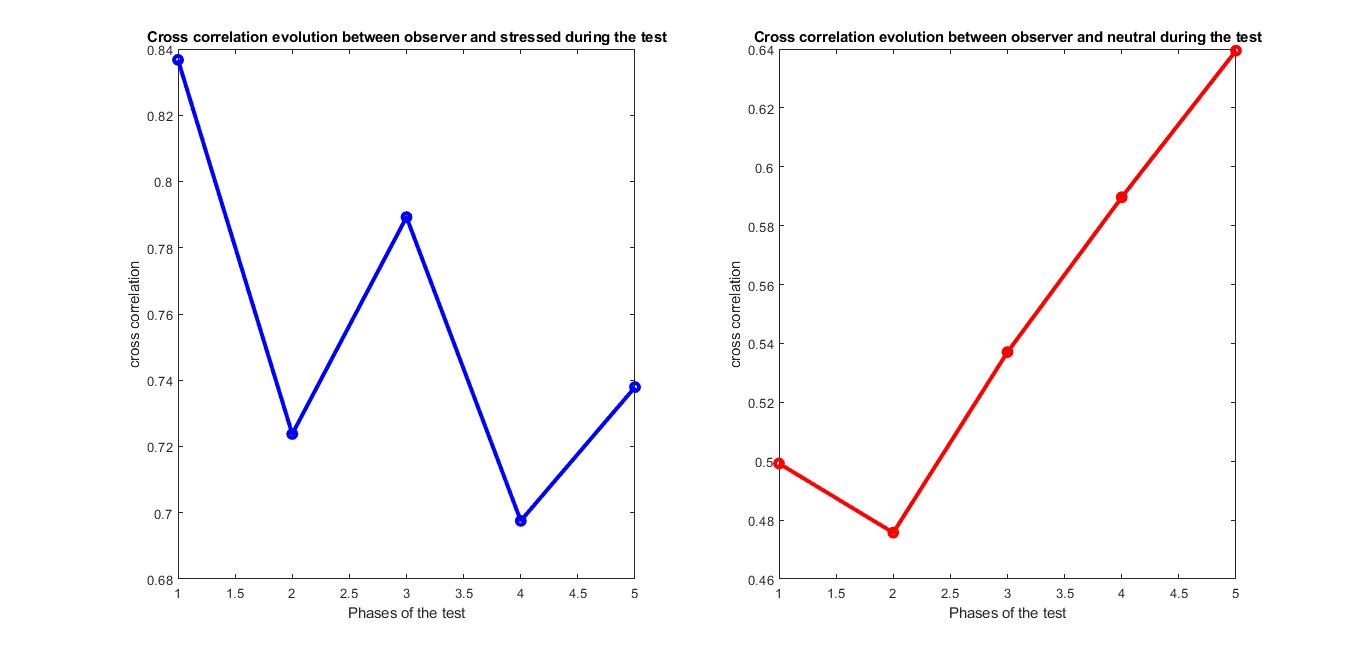
\includegraphics[scale=.28]{corr_time.jpg} 
	\end{center}  
	
	
\end{figure}

\end{frame}

\begin{frame}
\frametitle{Second dataset: correlation behaviour through time}


\begin{figure}[H]
	\begin{center}
		\hspace*{-1cm}
		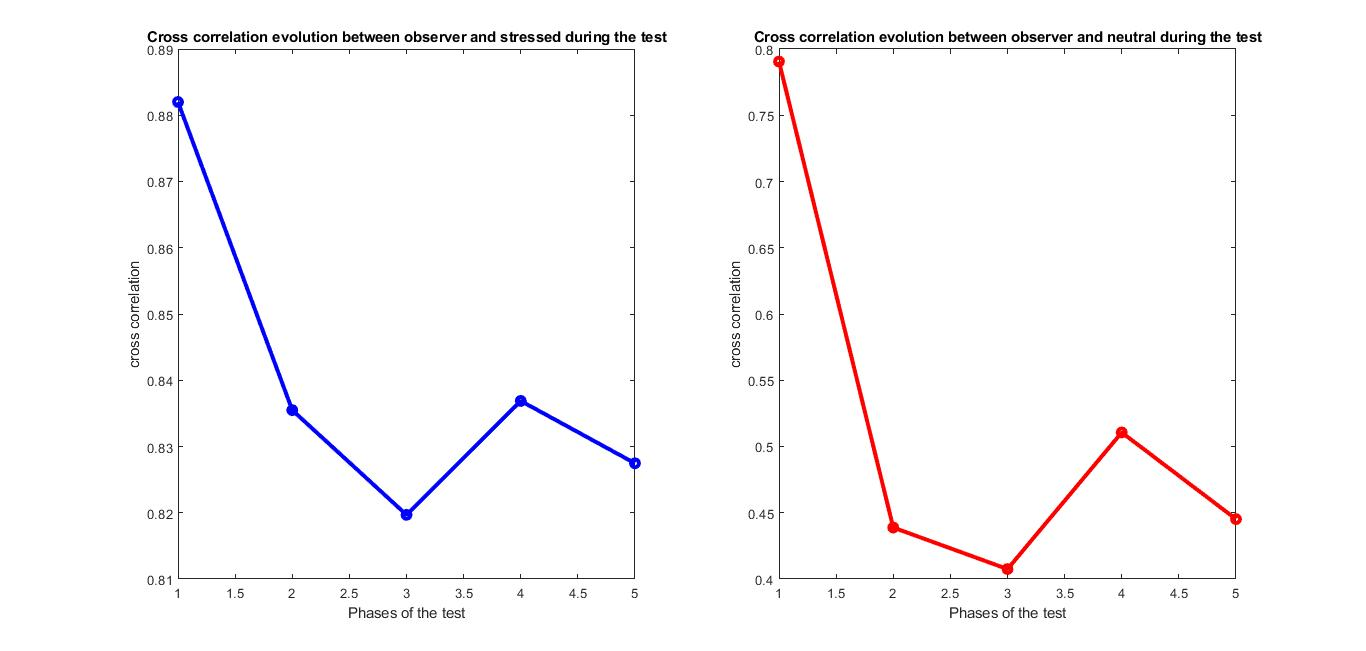
\includegraphics[scale=.28]{corr_time2.jpg} 
	\end{center}  
	
	
\end{figure}

\end{frame}

\begin{frame}
\frametitle{Third dataset: observer vs stressed and neutral}

Observer $95$ has been stressed for $30$ minutes.

\begin{figure}[H]
	\begin{center}
		\hspace*{-1cm}
		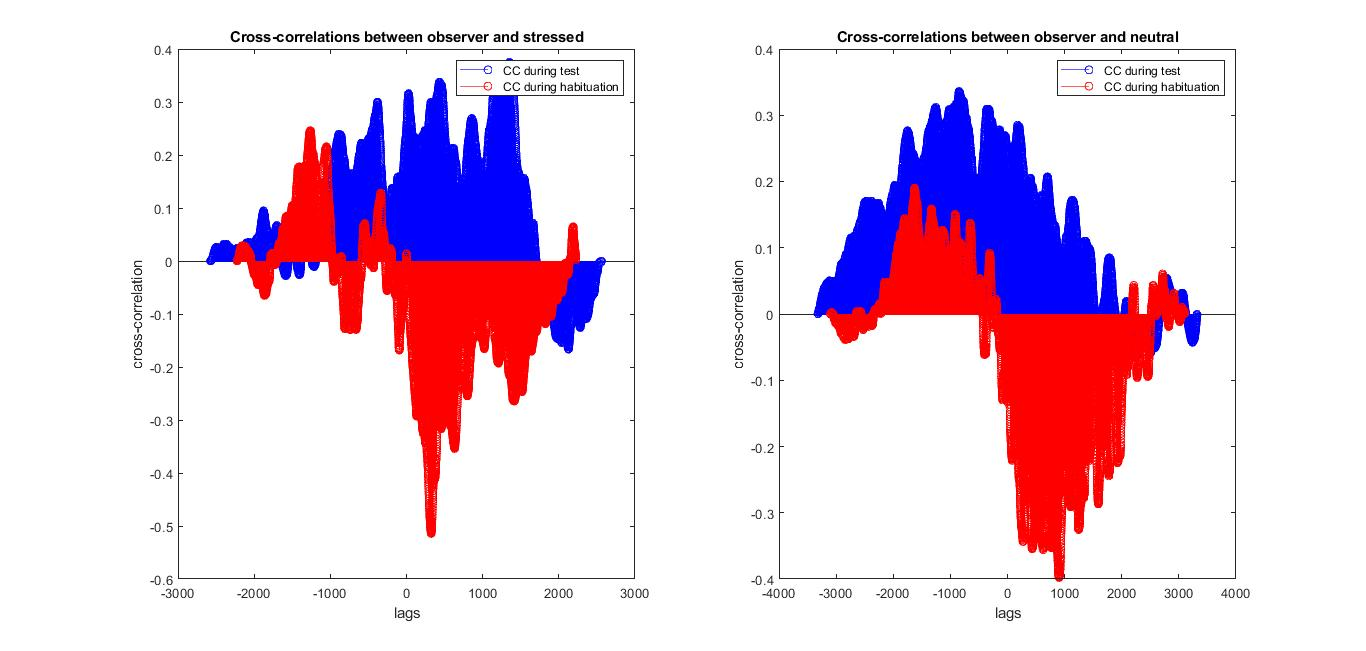
\includegraphics[scale=.30]{obs_stress_neut.jpg} 
	\end{center}  
	
	
\end{figure}

\end{frame}

\begin{frame}
\frametitle{Third dataset: observer vs stressed when distant}



\begin{figure}[H]
	\begin{center}
		\hspace*{-1cm}
		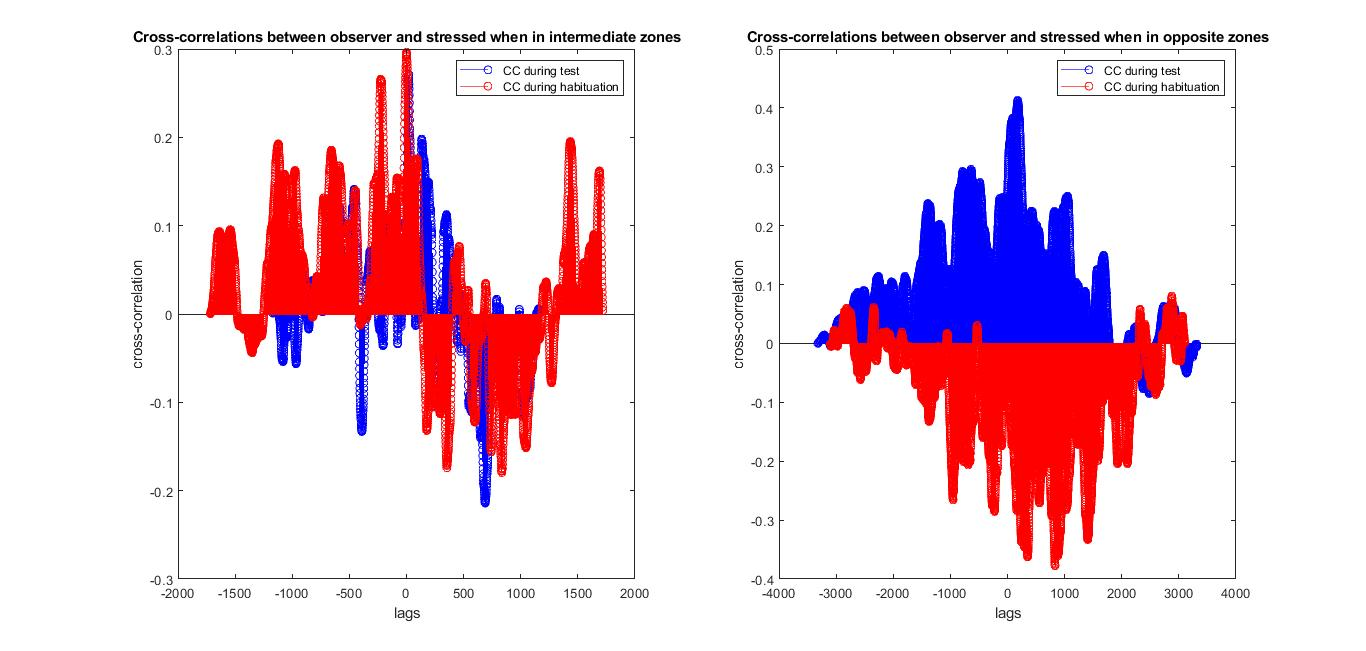
\includegraphics[scale=.30]{obs_stress_distant.jpg} 
	\end{center}  
	
	
\end{figure}

\end{frame}


\begin{frame}
\frametitle{Third dataset: observer vs neutral when distant}



\begin{figure}[H]
	\begin{center}
		\hspace*{-1cm}
		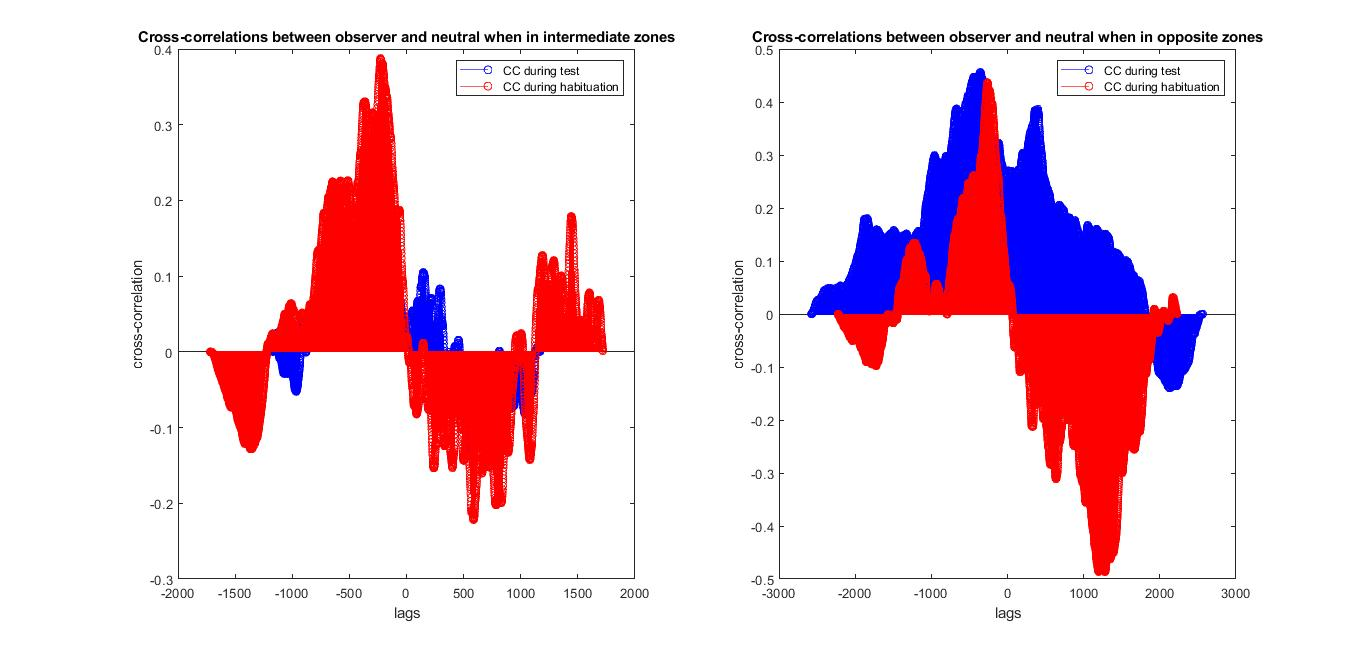
\includegraphics[scale=.30]{obs_neut_distant.jpg} 
	\end{center}  
	
	
\end{figure}

\end{frame}

\begin{frame}
\frametitle{Third dataset: correlation during sniffing}



\begin{figure}[H]
	\begin{center}
		\hspace*{-1cm}
		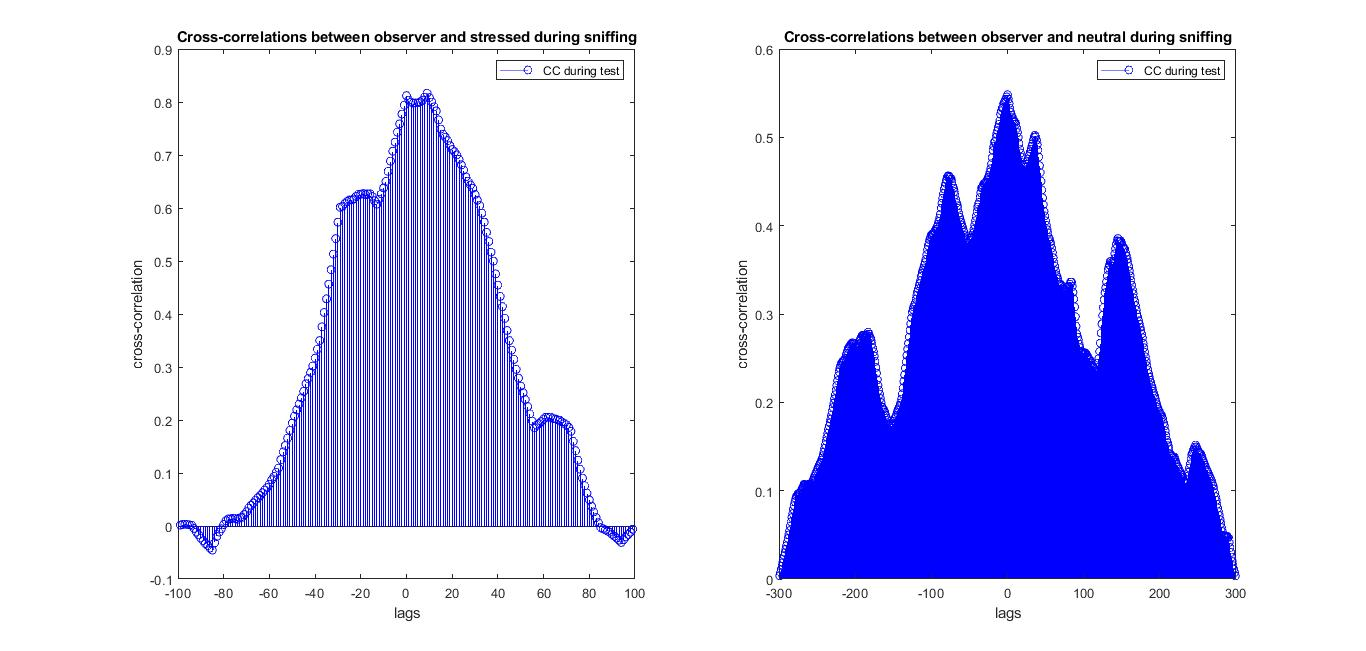
\includegraphics[scale=.30]{sniff3.jpg} 
	\end{center}  
	
	
\end{figure}

\end{frame}

\begin{frame}
\frametitle{Third dataset: correlation behaviour through time}


\begin{figure}[H]
	\begin{center}
		\hspace*{-1cm}
		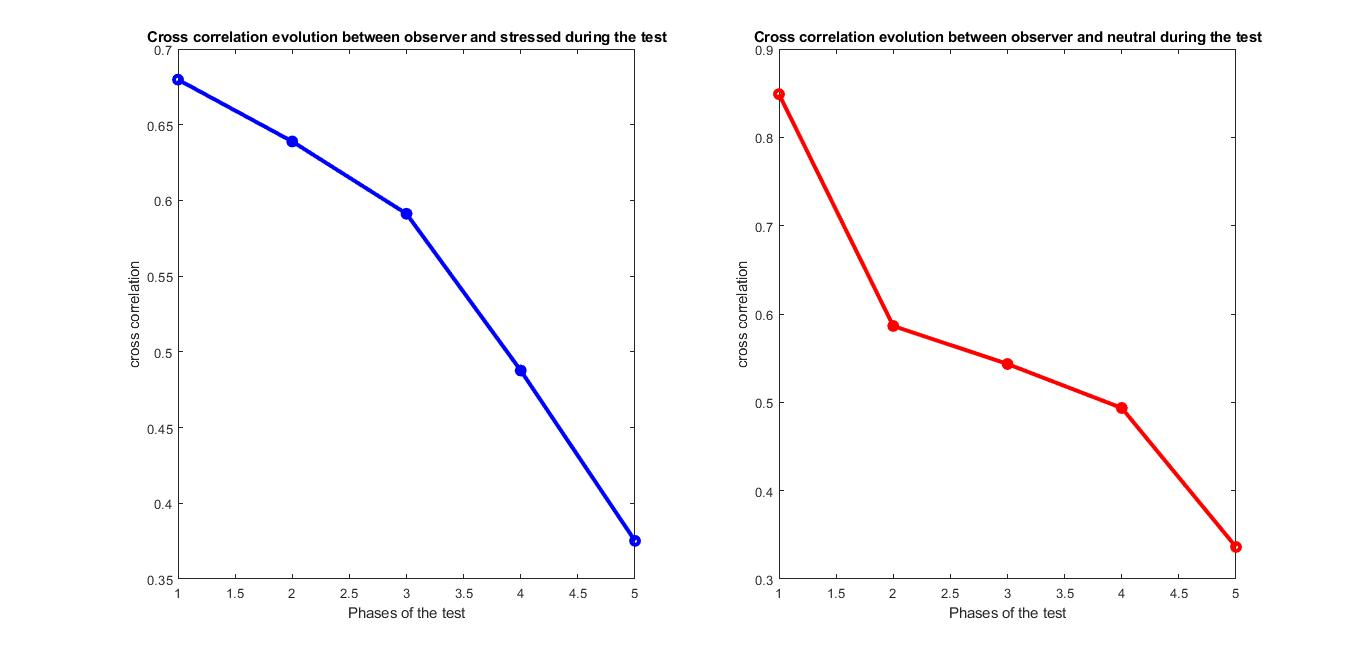
\includegraphics[scale=.28]{corr_time3.jpg} 
	\end{center}  
	
	
\end{figure}

\end{frame}

\begin{frame}
\frametitle{Third dataset: correlation during first interactions}


\begin{figure}[H]
	\begin{center}
		\hspace*{-1cm}
		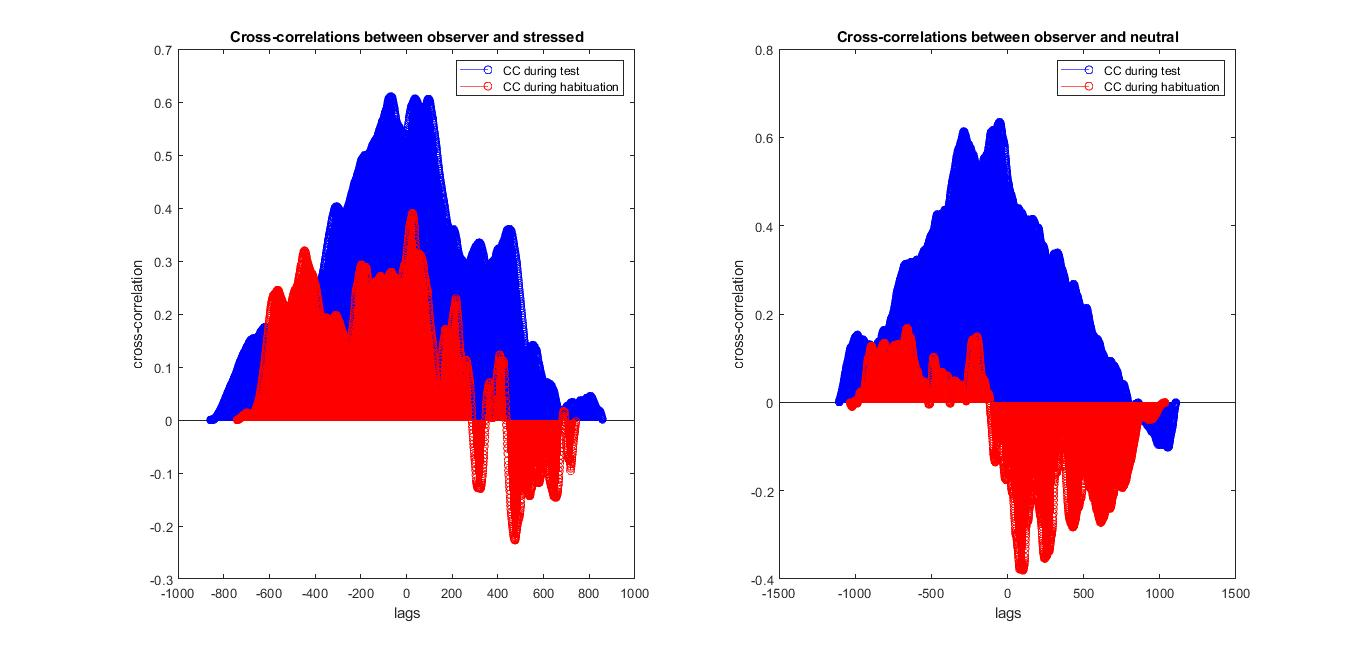
\includegraphics[scale=.28]{corr_reduced_times3.jpg} 
	\end{center}  
	
	
\end{figure}

\end{frame}

\begin{frame}
\frametitle{Third dataset: sniffing during first interactions}


\begin{figure}[H]
	\begin{center}
		\hspace*{-1cm}
		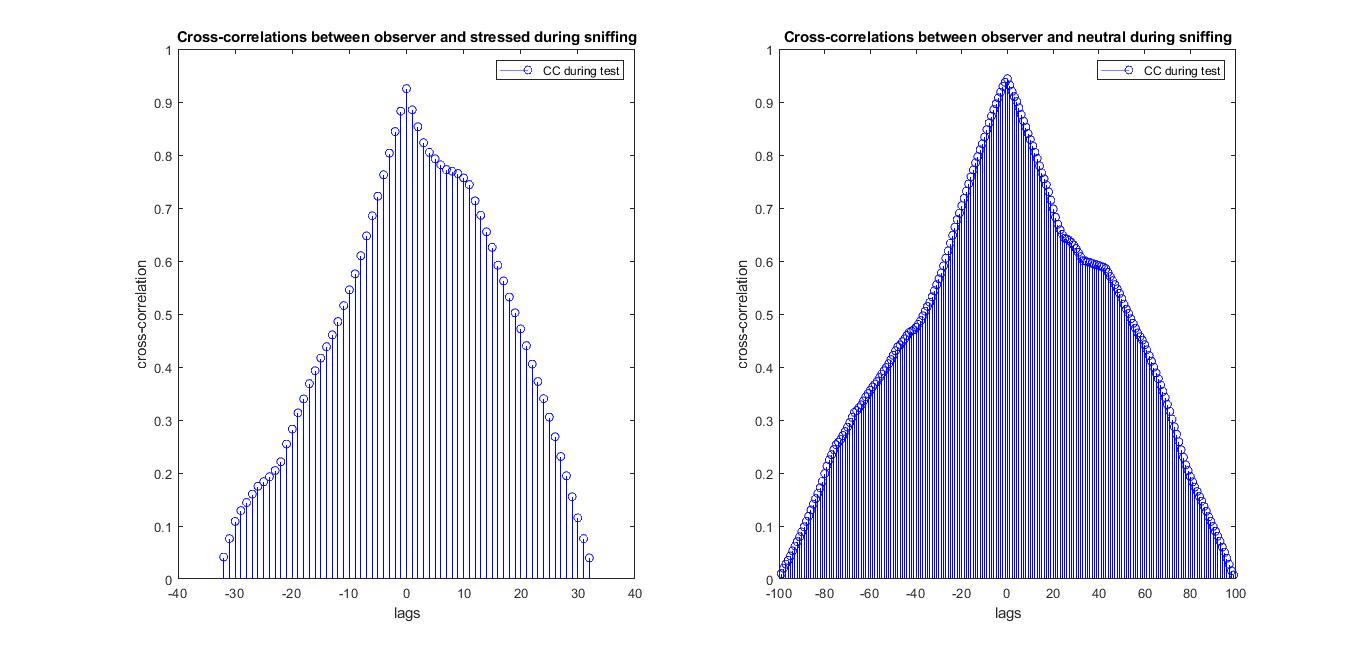
\includegraphics[scale=.28]{sniff3_reduced_times.jpg} 
	\end{center}  
	
	
\end{figure}

\end{frame}

\begin{frame}
\frametitle{Third dataset: pairs correlation with stressed during test}

Percentage of pairs showing correlation = $ 4.9\%$

\begin{figure}[H]
	\begin{center}
		\hspace*{-1cm}
		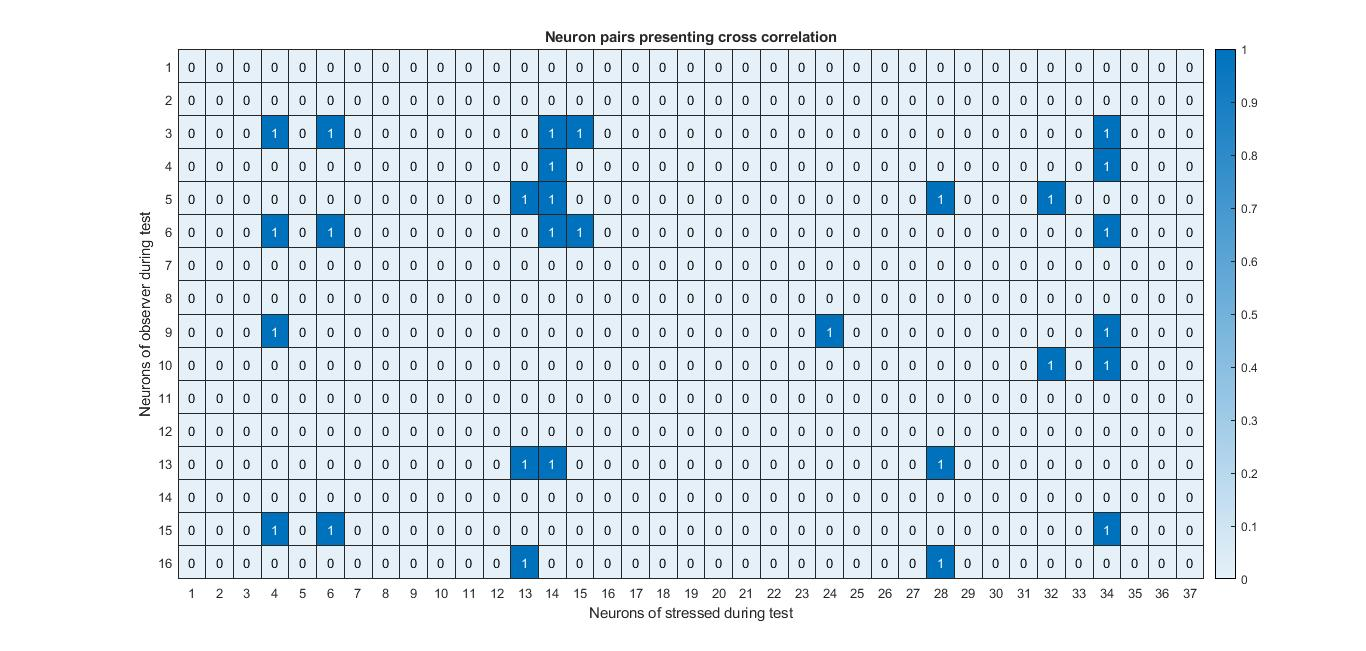
\includegraphics[scale=.28]{neuron_corr_stress_test3.jpg} 
	\end{center}  
	
	
\end{figure}

\end{frame}

\begin{frame}
\frametitle{Third dataset: pairs correlation with stressed during habituation}

Percentage of pairs showing correlation = $ 1.69\%$

\begin{figure}[H]
	\begin{center}
		\hspace*{-1cm}
		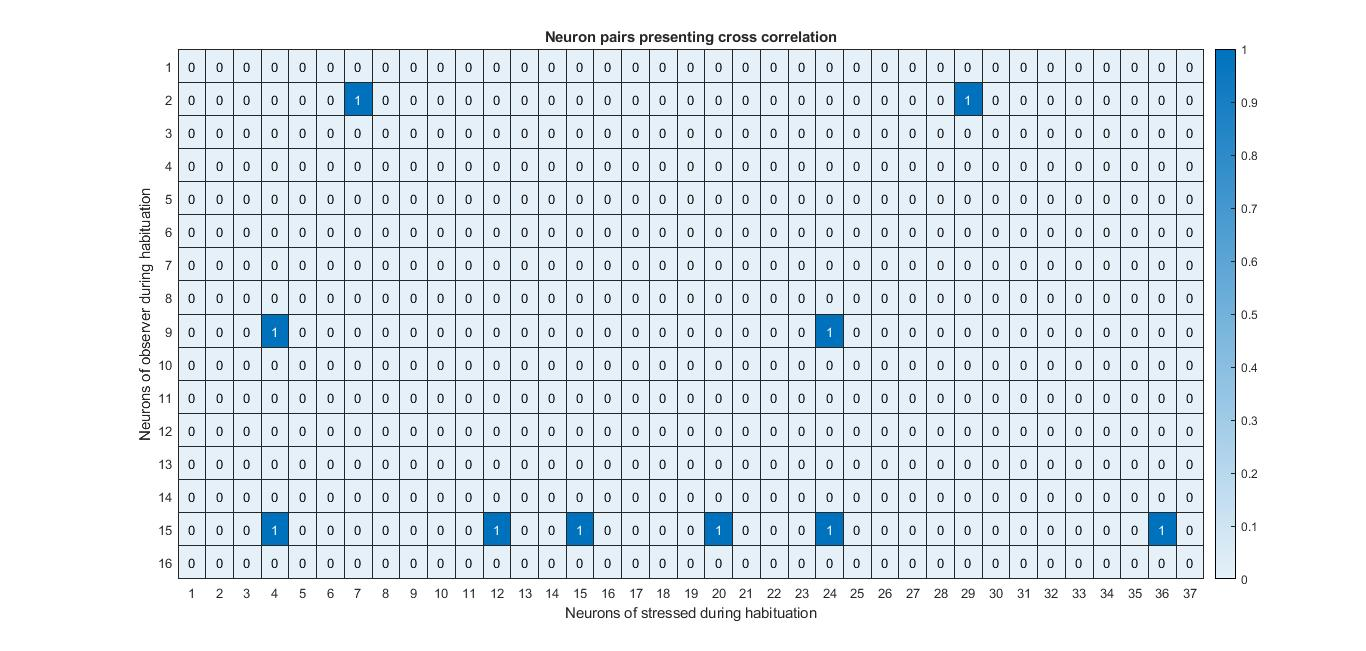
\includegraphics[scale=.28]{neuron_corr_stress_hab3.jpg} 
	\end{center}  
	
	
\end{figure}

\end{frame}

\begin{frame}
\frametitle{Third dataset: pairs correlation with neutral during test}

Percentage of pairs showing correlation = $ 14.7\%$

\begin{figure}[H]
	\begin{center}
		\hspace*{-1cm}
		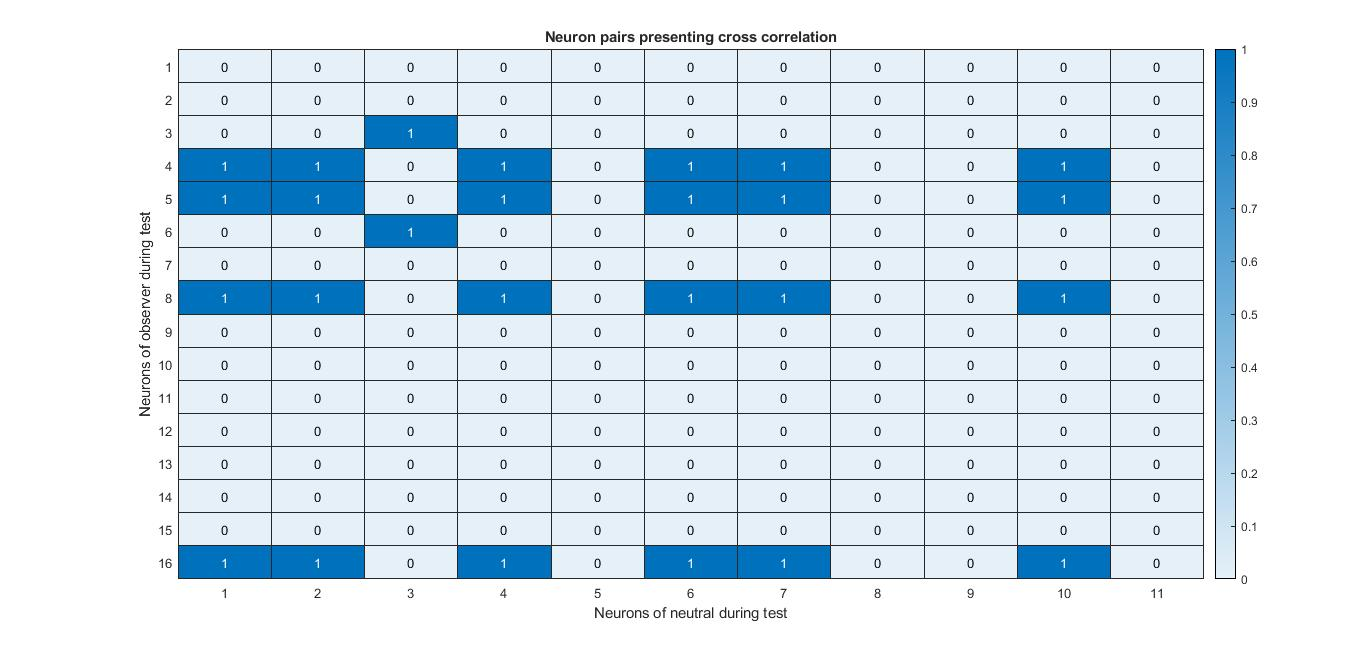
\includegraphics[scale=.28]{neuron_corr_neut_test3.jpg} 
	\end{center}  
	
	
\end{figure}

\end{frame}

\begin{frame}
\frametitle{Third dataset: pairs correlation with neutral during habituation}

Percentage of pairs showing correlation = $ 1.7\%$

\begin{figure}[H]
	\begin{center}
		\hspace*{-1cm}
		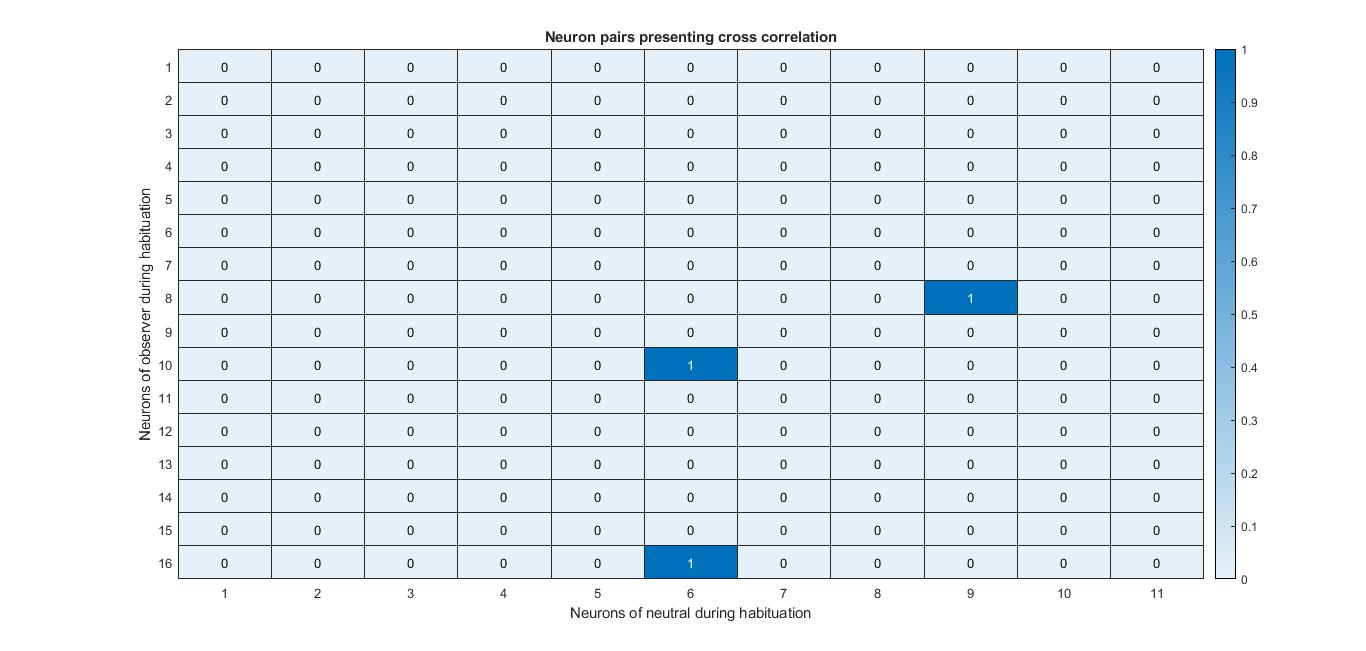
\includegraphics[scale=.28]{neuron_corr_neut_hab3.jpg} 
	\end{center}  
	
	
\end{figure}

\end{frame}








\begin{frame}
\frametitle{Fourth dataset: observer vs stressed and neutral}

Observer $105$ has been stressed for $30$ minutes.

\begin{figure}[H]
	\begin{center}
		\hspace*{-1cm}
		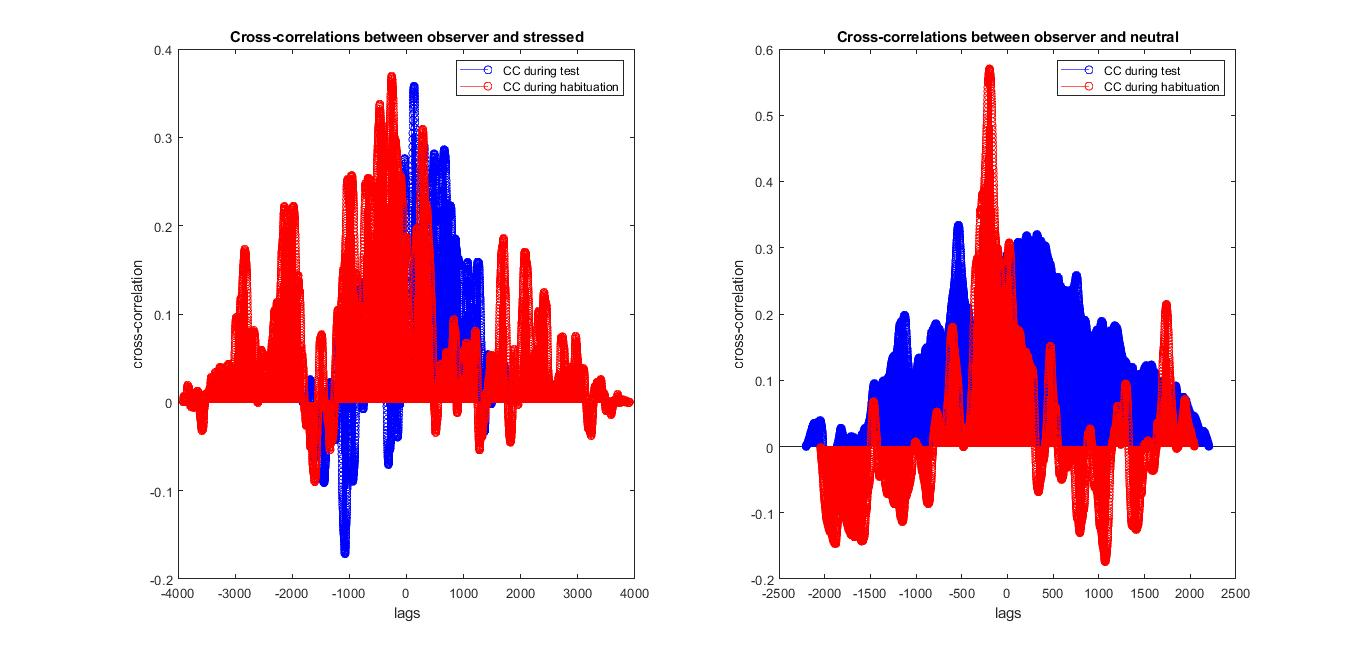
\includegraphics[scale=.30]{obs_stress_neut4.jpg} 
	\end{center}  
	
	
\end{figure}

\end{frame}




\begin{frame}
\frametitle{Fourth dataset: correlation behaviour through time}


\begin{figure}[H]
\begin{center}
\hspace*{-1cm}
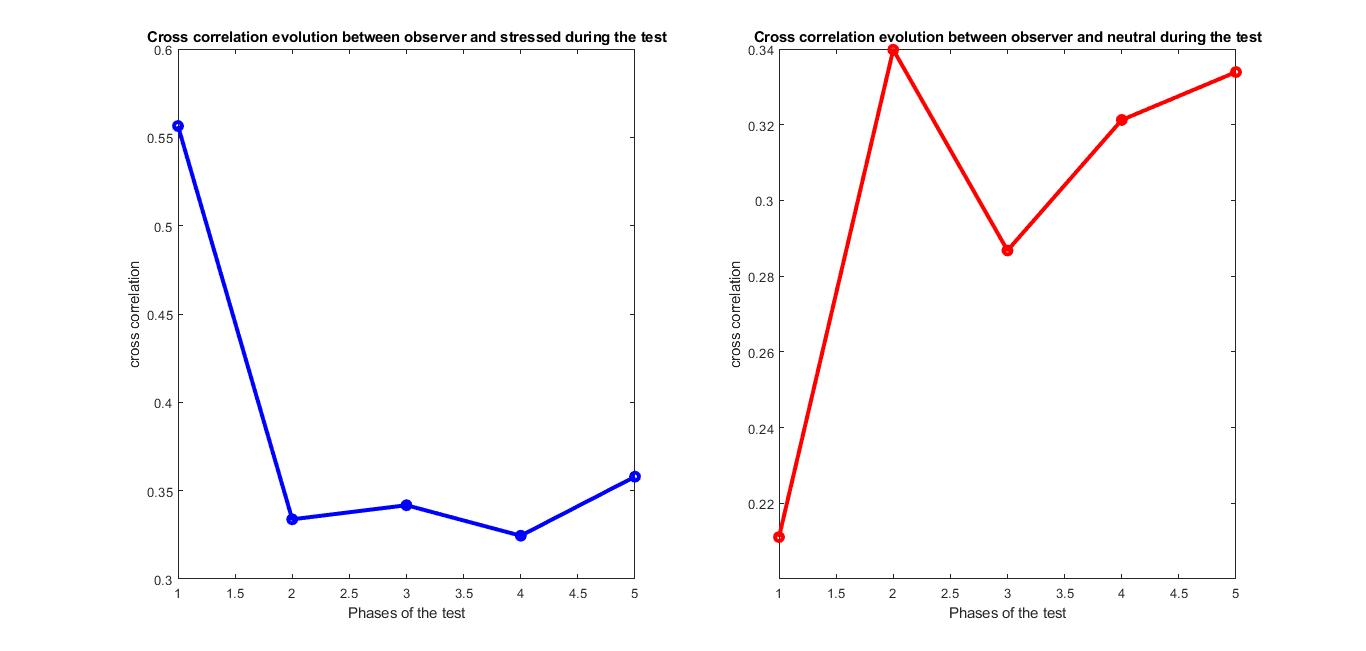
\includegraphics[scale=.28]{corr_time4.jpg} 
\end{center}  


\end{figure}

\end{frame}

\begin{frame}
\frametitle{Fourth dataset: pairs correlation with stressed during test}

Percentage of pairs showing correlation = $ 13.76\%$

\begin{figure}[H]
	\begin{center}
		\hspace*{-1cm}
		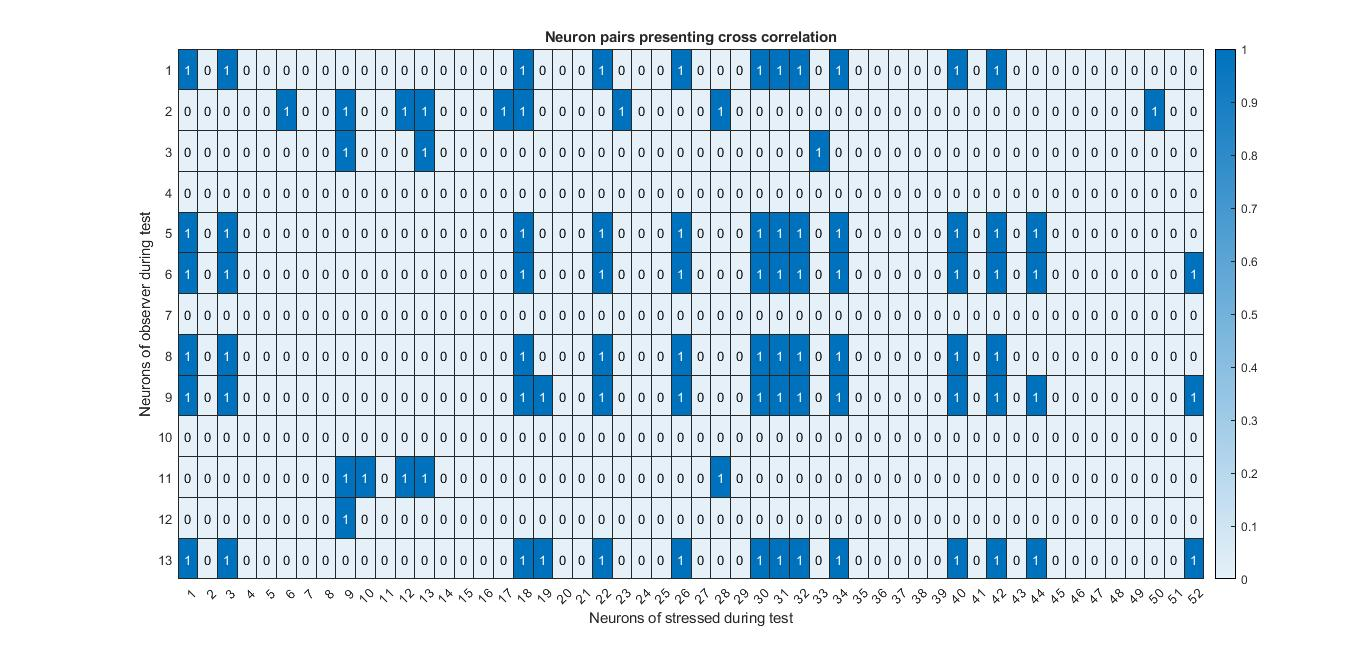
\includegraphics[scale=.28]{neuron_corr_stress_test4.jpg} 
	\end{center}  
	
	
\end{figure}

\end{frame}

\begin{frame}
\frametitle{Fourth dataset: pairs correlation with stressed during habituation}

Percentage of pairs showing correlation = $ 2.66\%$

\begin{figure}[H]
\begin{center}
	\hspace*{-1cm}
	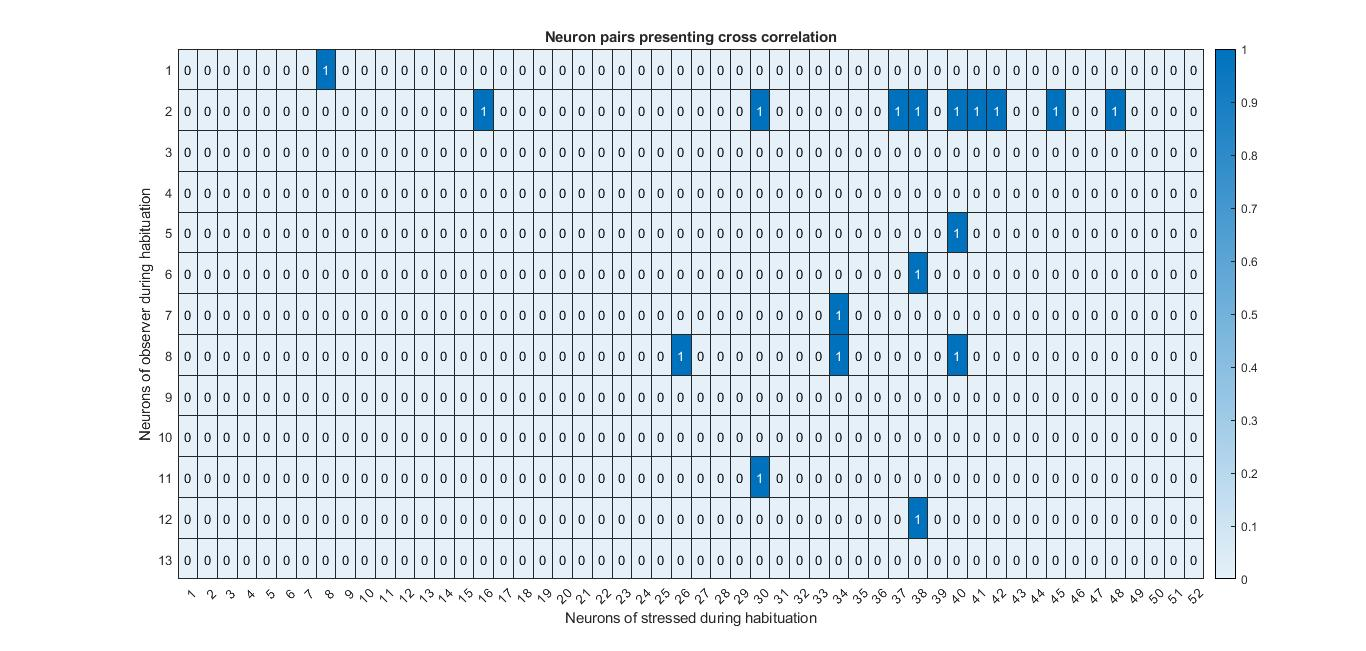
\includegraphics[scale=.28]{neuron_corr_stress_hab4.jpg} 
\end{center}  


\end{figure}

\end{frame}

\begin{frame}
\frametitle{Fourth dataset: pairs correlation with neutral during test}

Percentage of pairs showing correlation = $ 44.3\%$

\begin{figure}[H]
\begin{center}
\hspace*{-1cm}
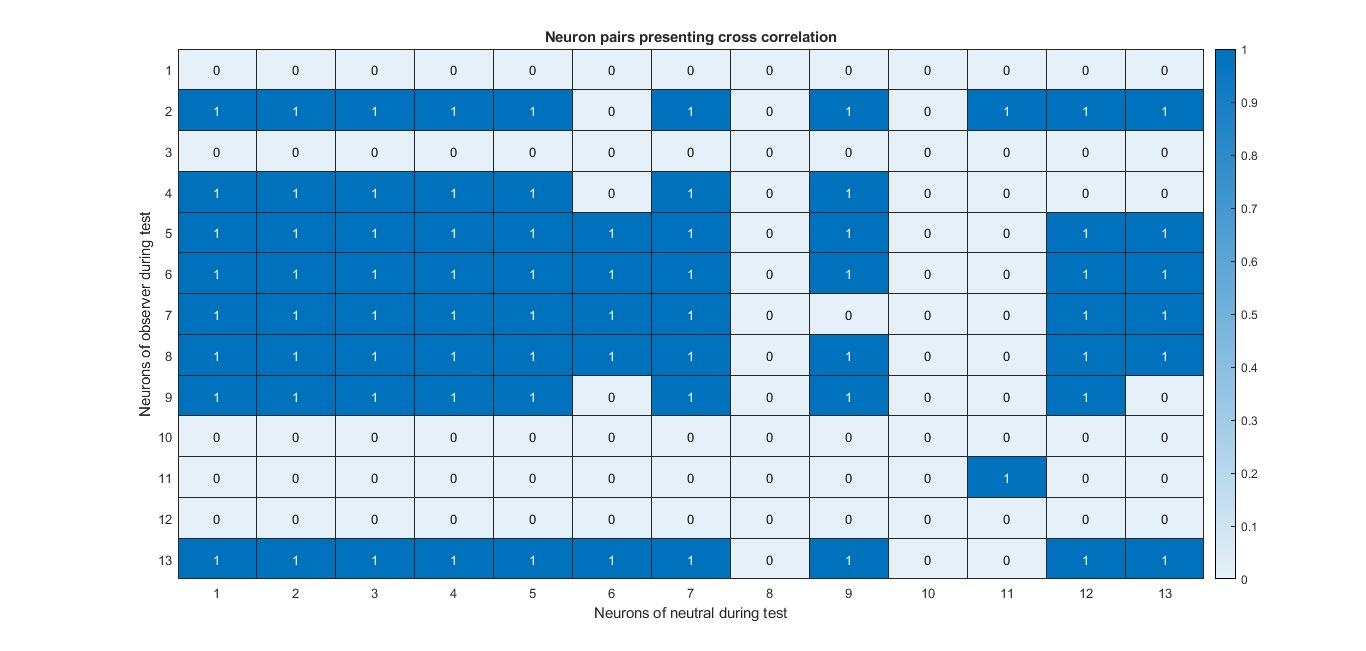
\includegraphics[scale=.28]{neuron_corr_neut_test4.jpg} 
\end{center}  


\end{figure}

\end{frame}

\begin{frame}
\frametitle{Fourth dataset: pairs correlation with neutral during habituation}

Percentage of pairs showing correlation = $ 18.9\%$

\begin{figure}[H]
\begin{center}
\hspace*{-1cm}
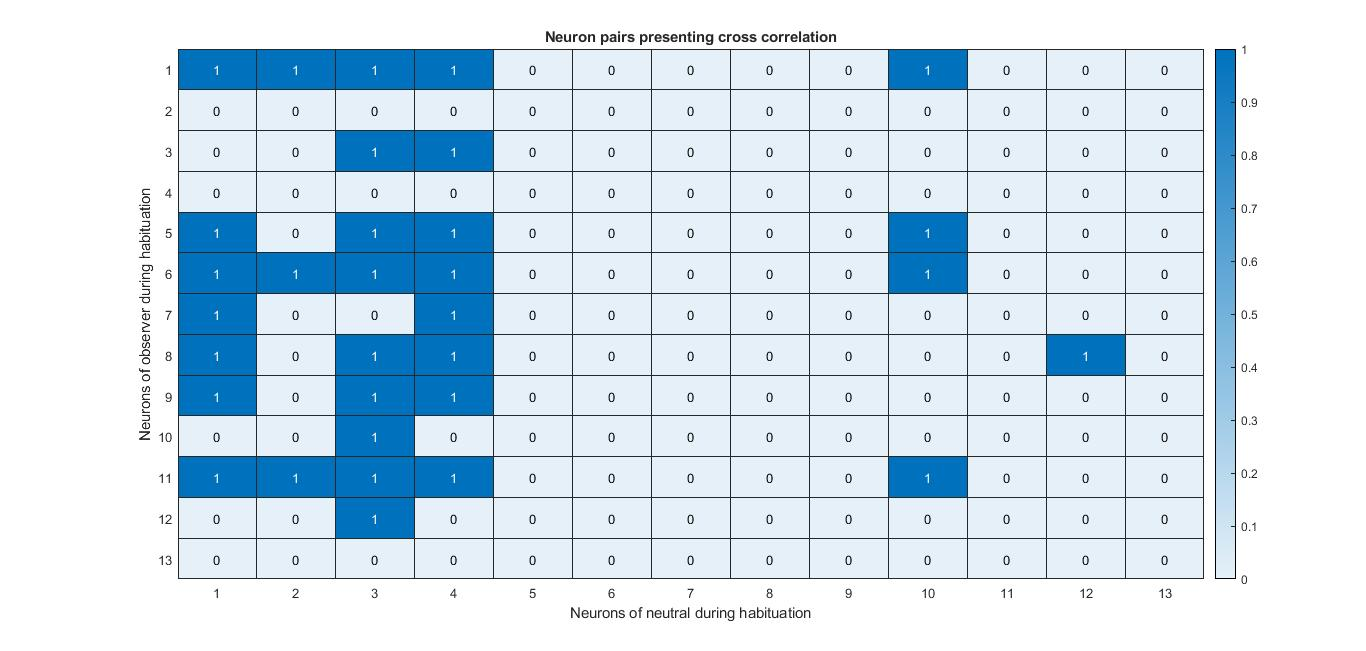
\includegraphics[scale=.28]{neuron_corr_neut_hab4.jpg} 
\end{center}  


\end{figure}

\end{frame}



\begin{frame}
\frametitle{Conclusion on third and fourth datasets}

\begin{itemize}
	\item Considering the overall interaction periods, for stressed observers the correlation between mice is not particularly different in the test compared to the habituation, in contrast with first and second datasets
	
	\item However, especially for the third dataset, there is still  higher correlation if we consider the first part of the interaction, i.e. stressed observers seem to have "shorter memory"
	
	\item Highest correlation is still obtained when considering the sniffing period
	
	\item Good correlation in the test rather than the habituation is still obtained if we consider single neuronal pairs
\end{itemize}
\end{frame}



\begin{frame}
\frametitle{Average statistics on all datasets}

In the following, summarizing statistics (computed as average of all datasets) are provided.\\
Other informations about similarity between signals can be also obtained from the following quantities:
\vspace{1 cm}
\begin{itemize}
	\item \textbf{Infinity error}:
	$$||f(t) - g(t)||_\infty = sup\{ |f(t)-g(t)| : t \in [t_1,t_2]\}$$
	
	\item \textbf{$L^2$ error}:
	
	$$||f(t) - g(t)||_{L^2} = \int_{t_1}^{t_2}|f(t)-g(t)|^2 dt$$
	

\end{itemize}
\end{frame}


\begin{frame}
\frametitle{Infinity errors between observer and stressed}



\begin{figure}[H]
	\begin{center}
		\hspace*{-1.7cm}
		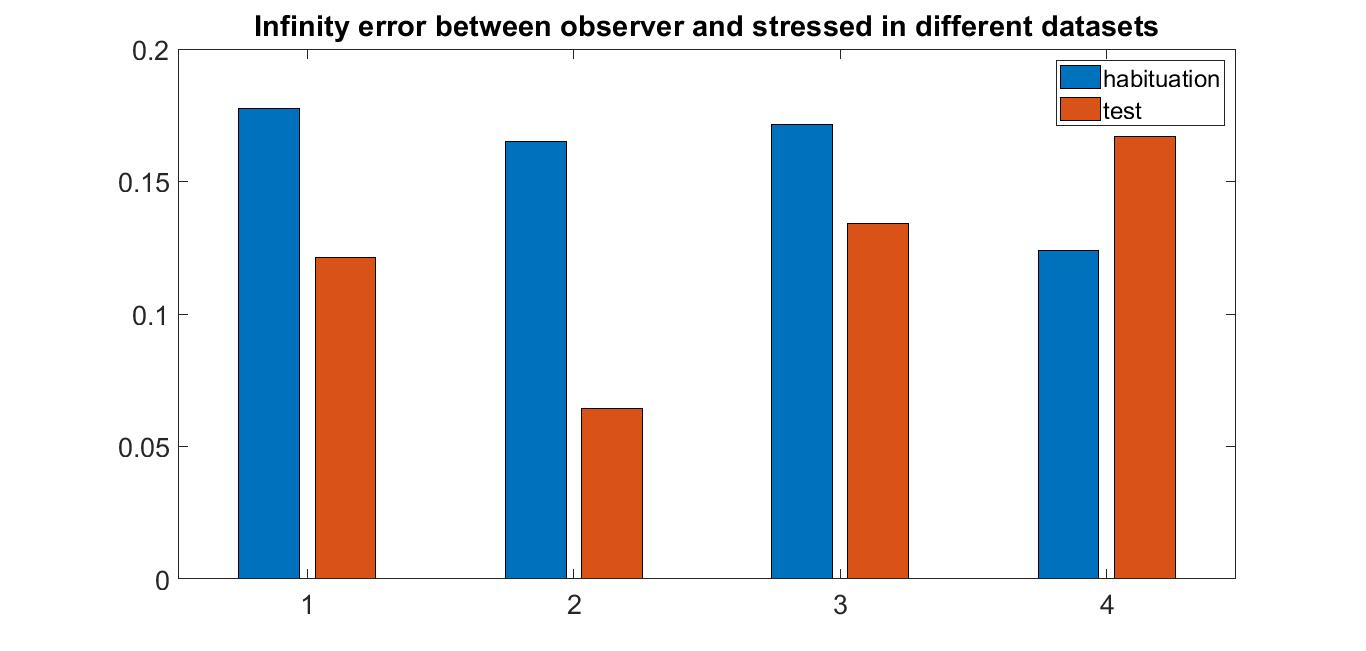
\includegraphics[scale=.32]{inf_err_stress.jpg} 
	\end{center}  
	
	
\end{figure}

\end{frame}

\begin{frame}
\frametitle{Infinity errors between observer and neutral}



\begin{figure}[H]
\begin{center}
	\hspace*{-1.7cm}
	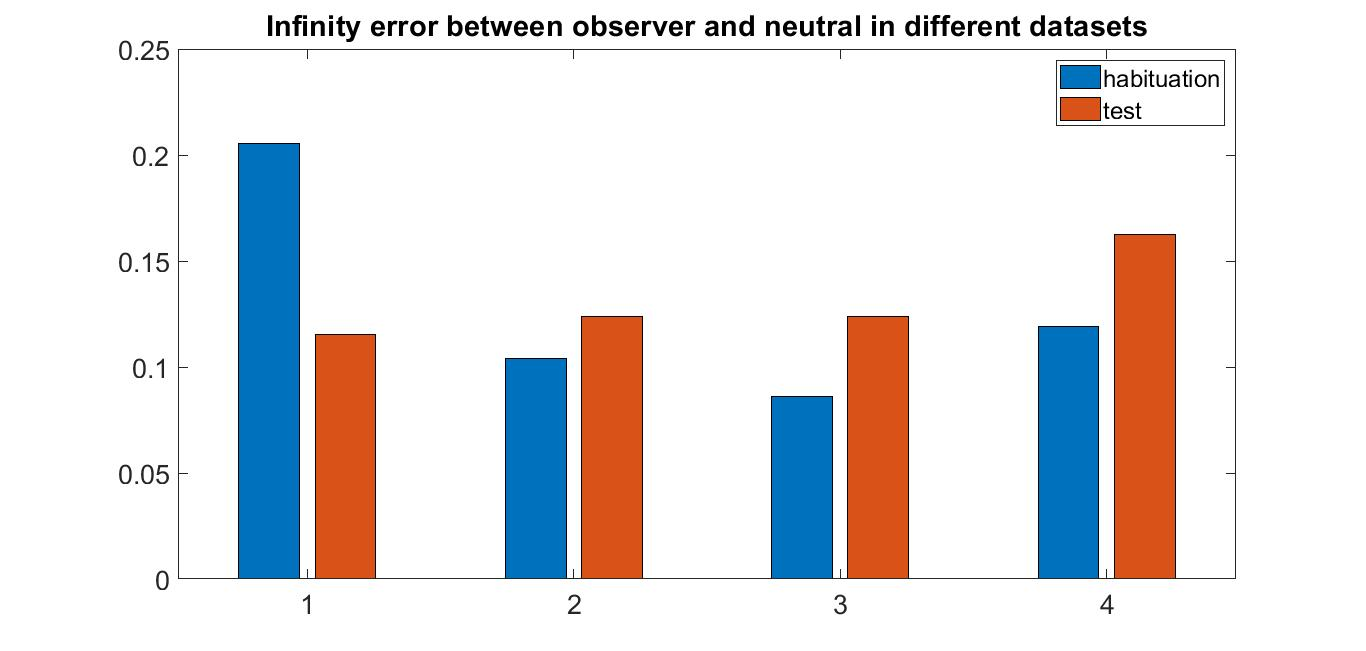
\includegraphics[scale=.32]{inf_erro_neut.jpg} 
\end{center}  


\end{figure}

\end{frame}

\begin{frame}
\frametitle{Average Infinity errors with neutral observer}

\begin{figure}[H]
	\begin{center}
		\hspace*{-1.7cm}
		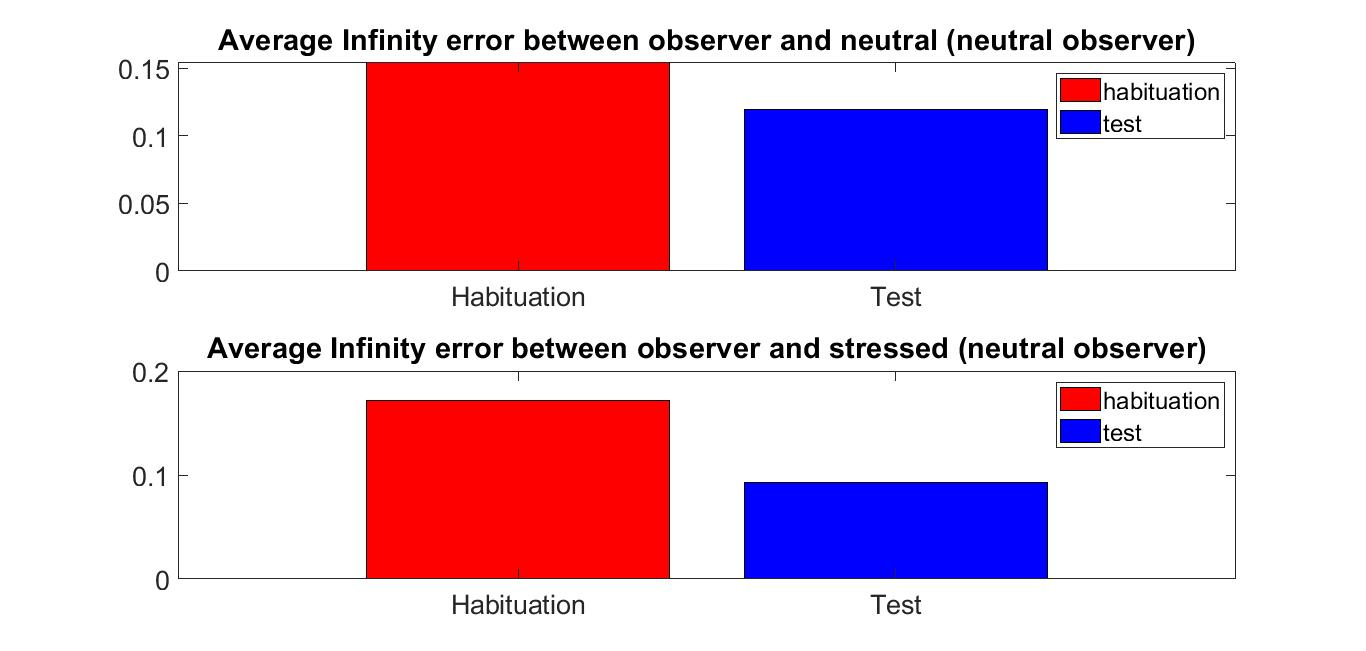
\includegraphics[scale=.32]{avg_inf.jpg} 
	\end{center}  
	
	
\end{figure}


\end{frame}

\begin{frame}
\frametitle{Average Infinity errors with stressed observer}

\begin{figure}[H]
	\begin{center}
		\hspace*{-1.7cm}
		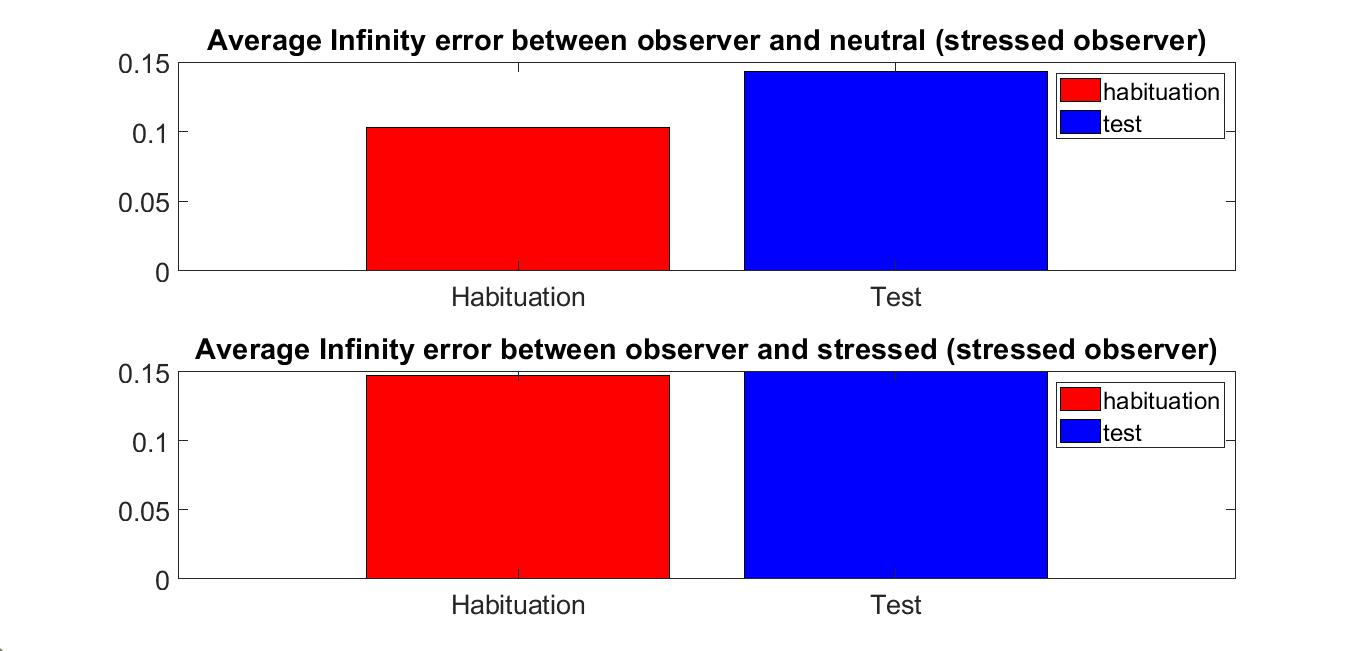
\includegraphics[scale=.32]{avg_inf2.jpg} 
	\end{center}  
	
	
\end{figure}


\end{frame}




\begin{frame}
\frametitle{ $L^2$ errors between observer and stressed}



\begin{figure}[H]
	\begin{center}
		\hspace*{-1.7cm}
		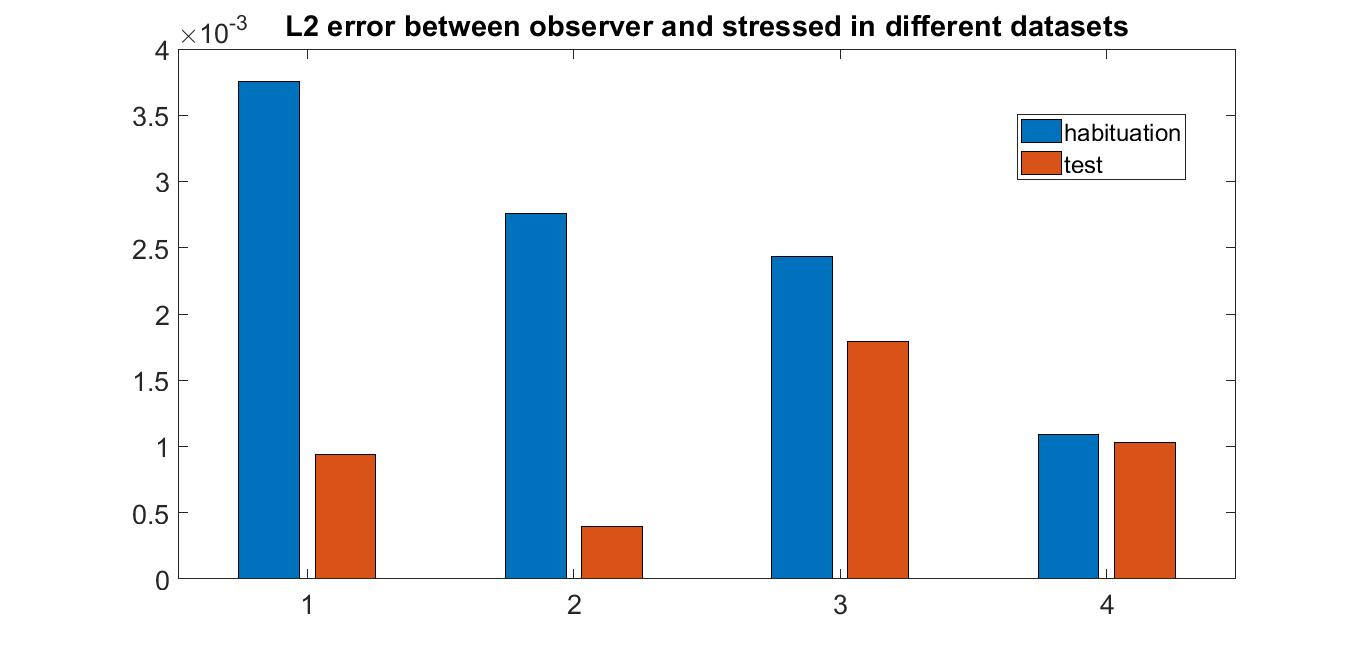
\includegraphics[scale=.32]{L2_err_stress.jpg} 
	\end{center}  
	
	
\end{figure}

\end{frame}

\begin{frame}
\frametitle{ $L^2$ errors between observer and neutral}



\begin{figure}[H]
\begin{center}
	\hspace*{-1.7cm}
	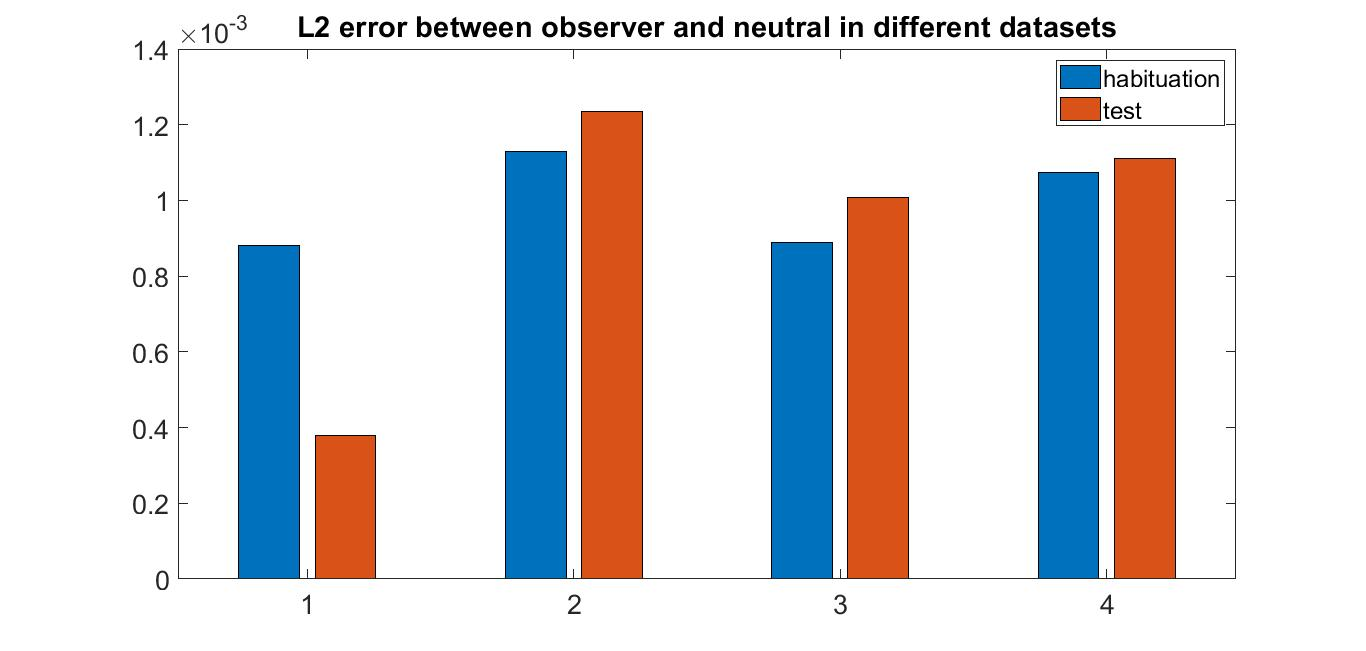
\includegraphics[scale=.32]{L2_err_neut.jpg} 
\end{center}  


\end{figure}

\end{frame}


\begin{frame}
\frametitle{Average $L^2$ errors with neutral observer}


\begin{figure}[H]
	\begin{center}
		\hspace*{-1.7cm}
		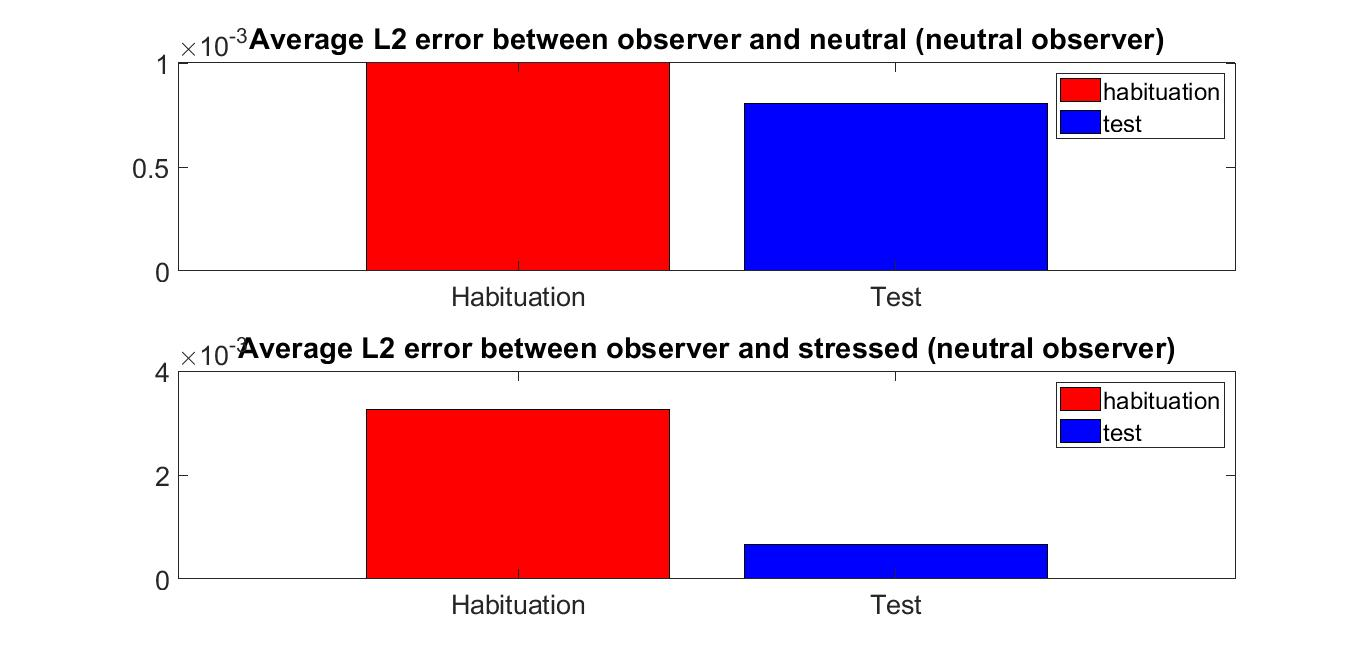
\includegraphics[scale=.32]{avg_L2.jpg} 
	\end{center}  
	
	
\end{figure}



\end{frame}

\begin{frame}
\frametitle{Average $L^2$ errors with stressed observer}


\begin{figure}[H]
	\begin{center}
		\hspace*{-1.7cm}
		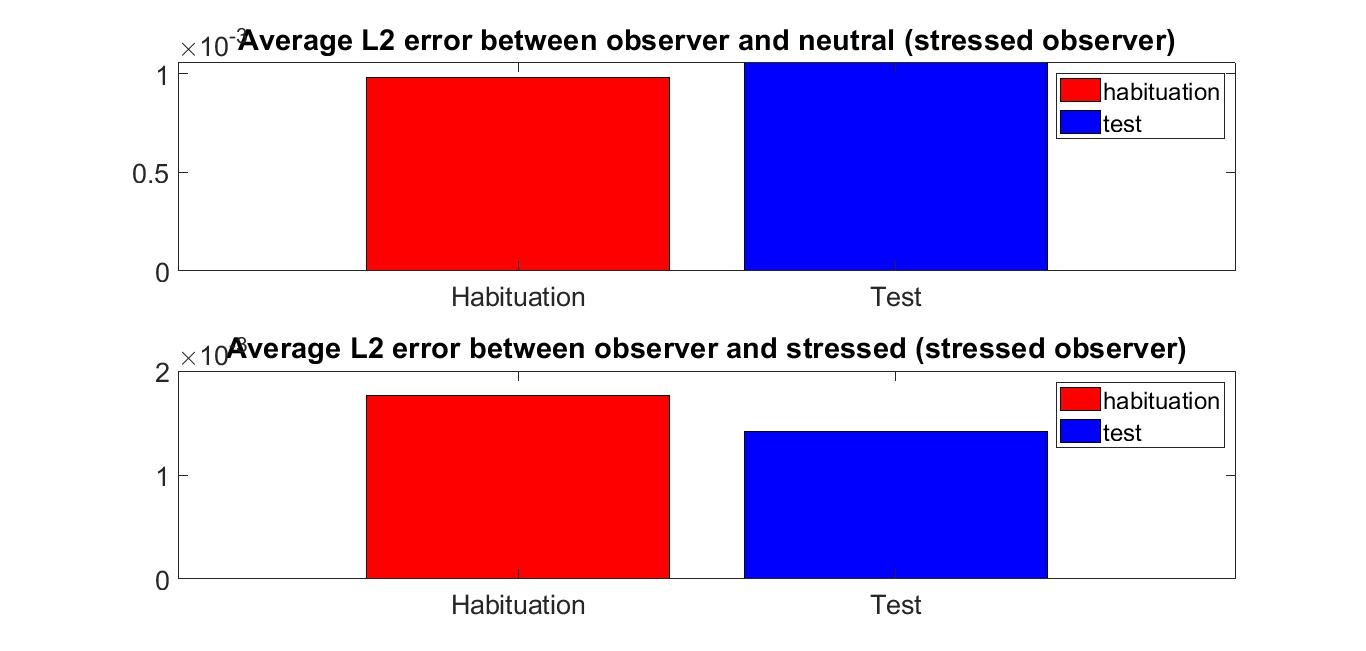
\includegraphics[scale=.32]{avg_L22.jpg} 
	\end{center}  
	
	
\end{figure}



\end{frame}


\begin{frame}
\frametitle{ Correlations between observer and stressed}



\begin{figure}[H]
	\begin{center}
		\hspace*{-1.7cm}
		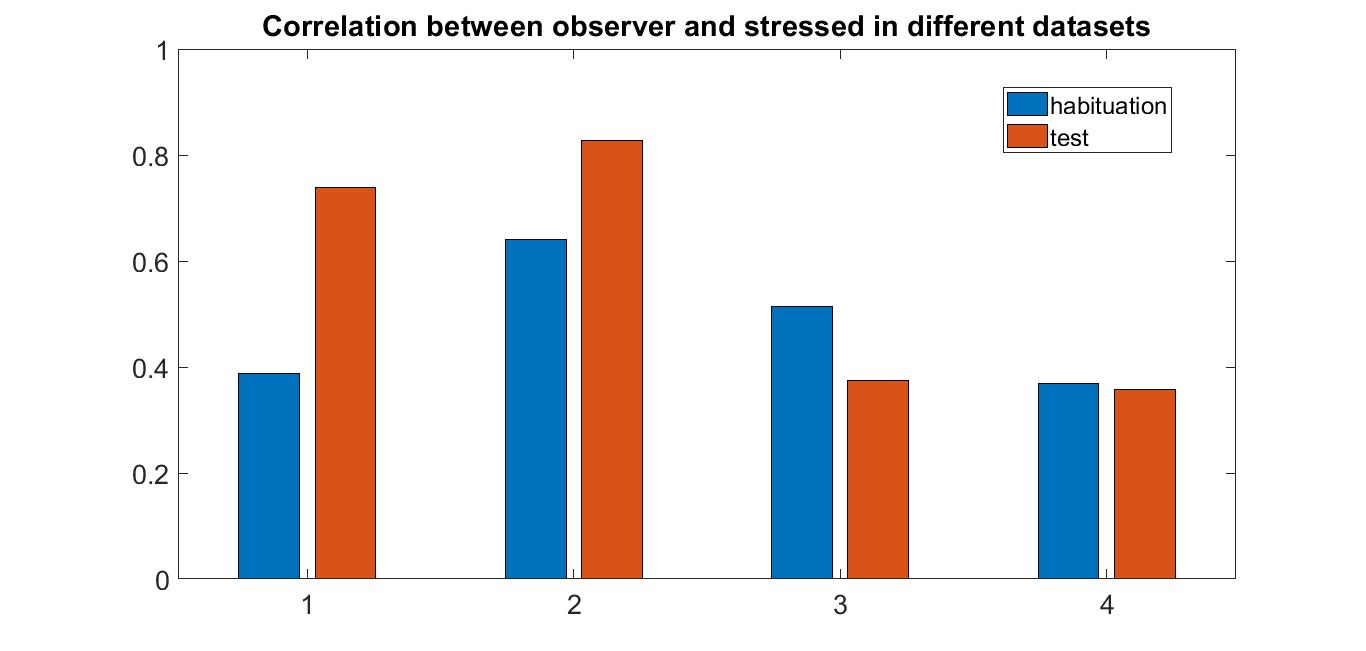
\includegraphics[scale=.32]{corr_bar_stress.jpg} 
	\end{center}  
	
	
\end{figure}

\end{frame}

\begin{frame}
\frametitle{ Correlations between observer and neutral}



\begin{figure}[H]
	\begin{center}
		\hspace*{-1.7cm}
		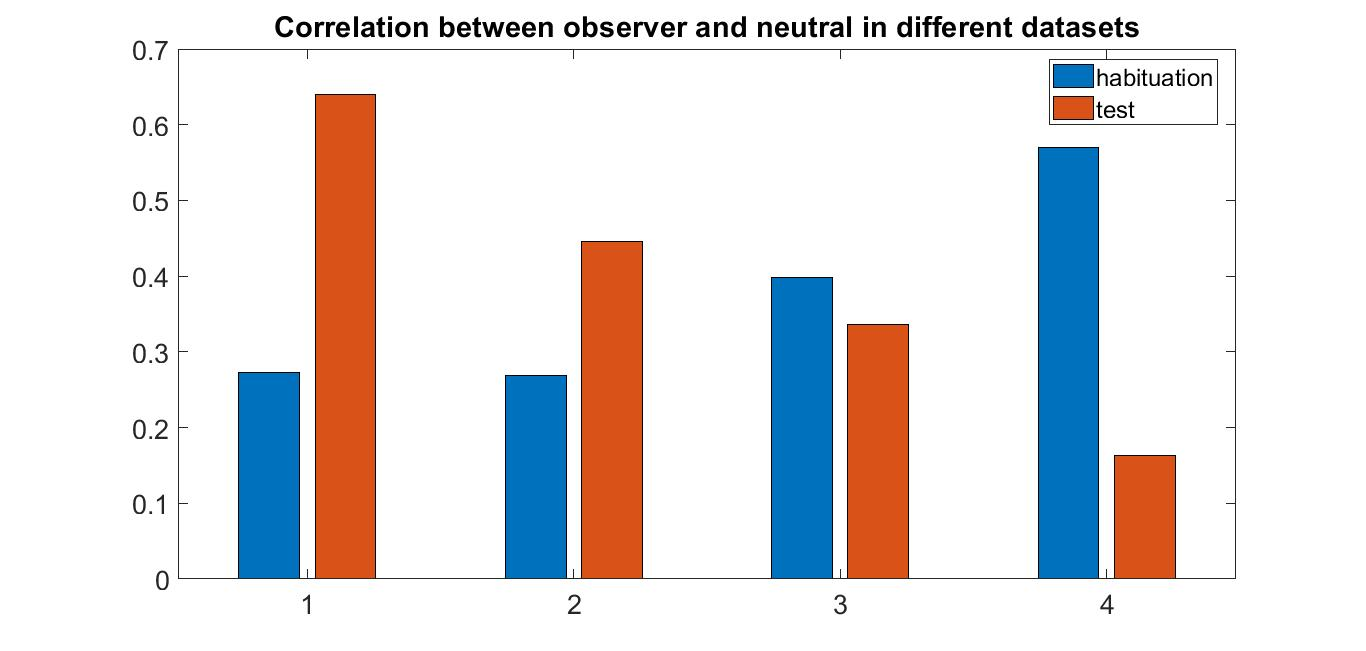
\includegraphics[scale=.32]{corr_bar_neut.jpg} 
	\end{center}  
	
	
\end{figure}

\end{frame}

\begin{frame}
\frametitle{ Correlations between observer and stressed during first interactions}



\begin{figure}[H]
	\begin{center}
		\hspace*{-1.7cm}
		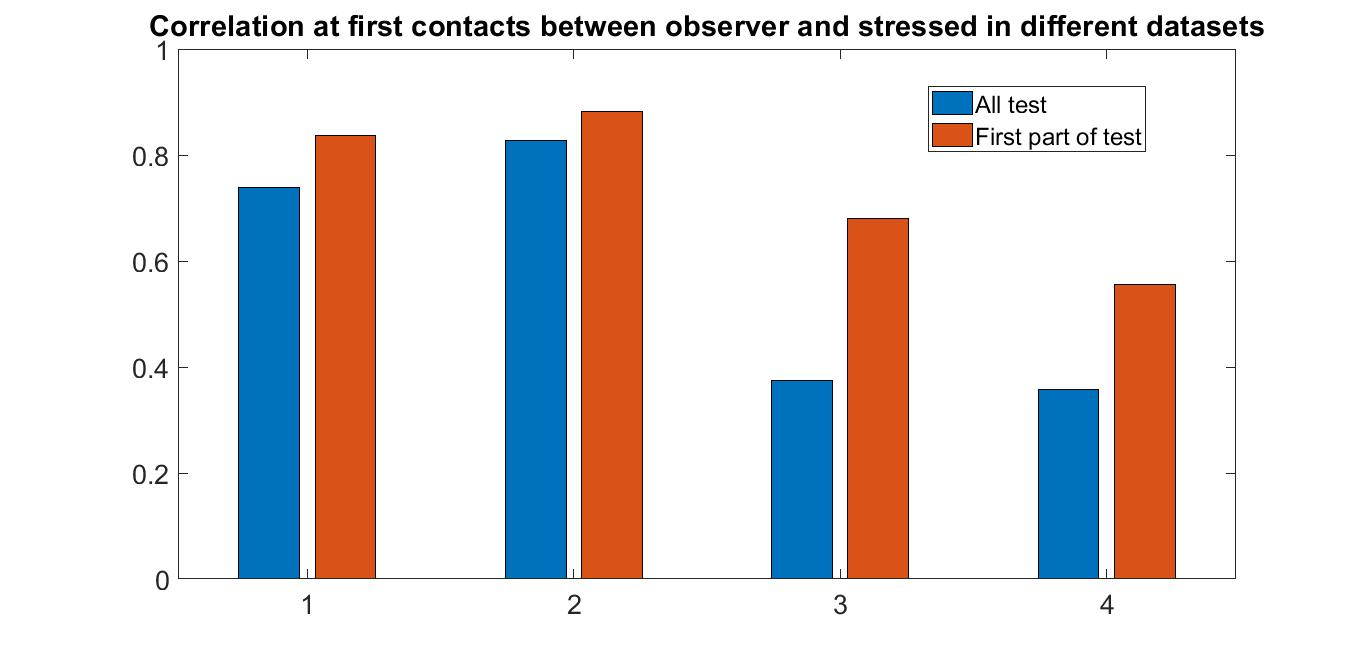
\includegraphics[scale=.32]{corr_bar_contact_stress.jpg} 
	\end{center}  
	
	
\end{figure}

\end{frame}

\begin{frame}
\frametitle{ Correlations between observer and neutral during first interactions}



\begin{figure}[H]
	\begin{center}
		\hspace*{-1.7cm}
		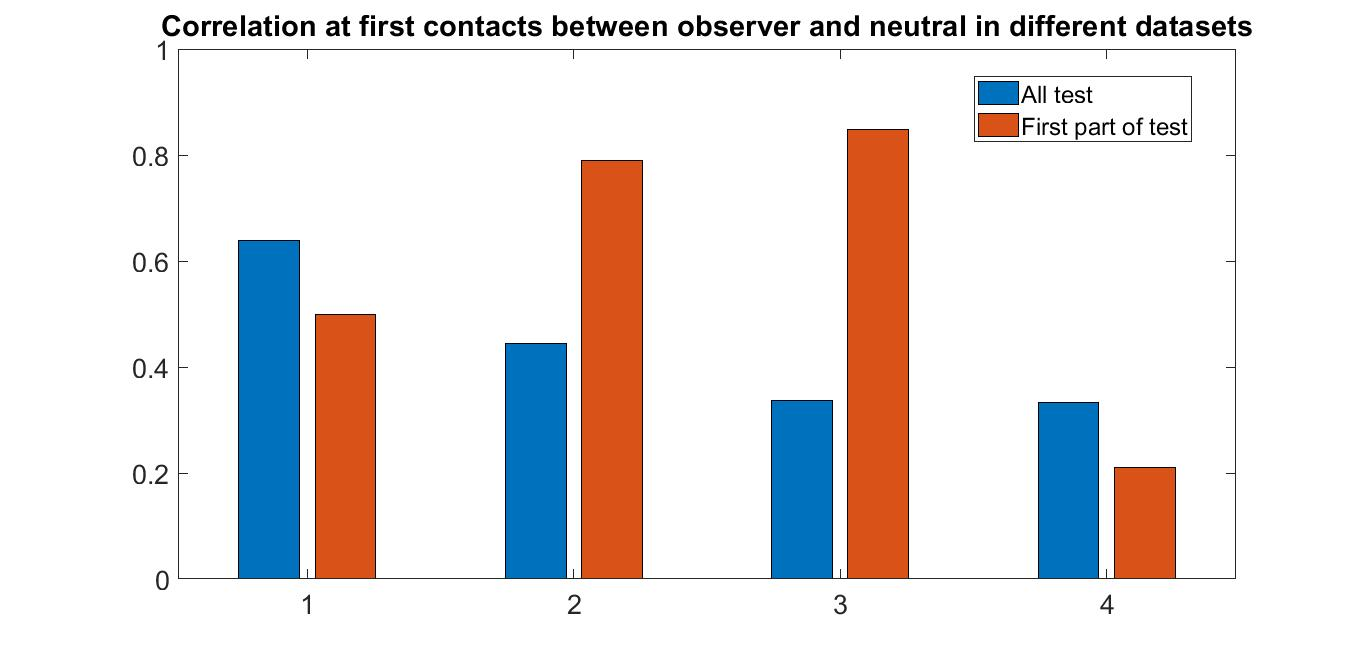
\includegraphics[scale=.32]{corr_bar_contact_neut.jpg} 
	\end{center}  
	
	
\end{figure}

\end{frame}

\begin{frame}
\frametitle{ Average correlation between observer and stressed with neutral observer}



\begin{figure}[H]
	\begin{center}
		\hspace*{-1.7cm}
		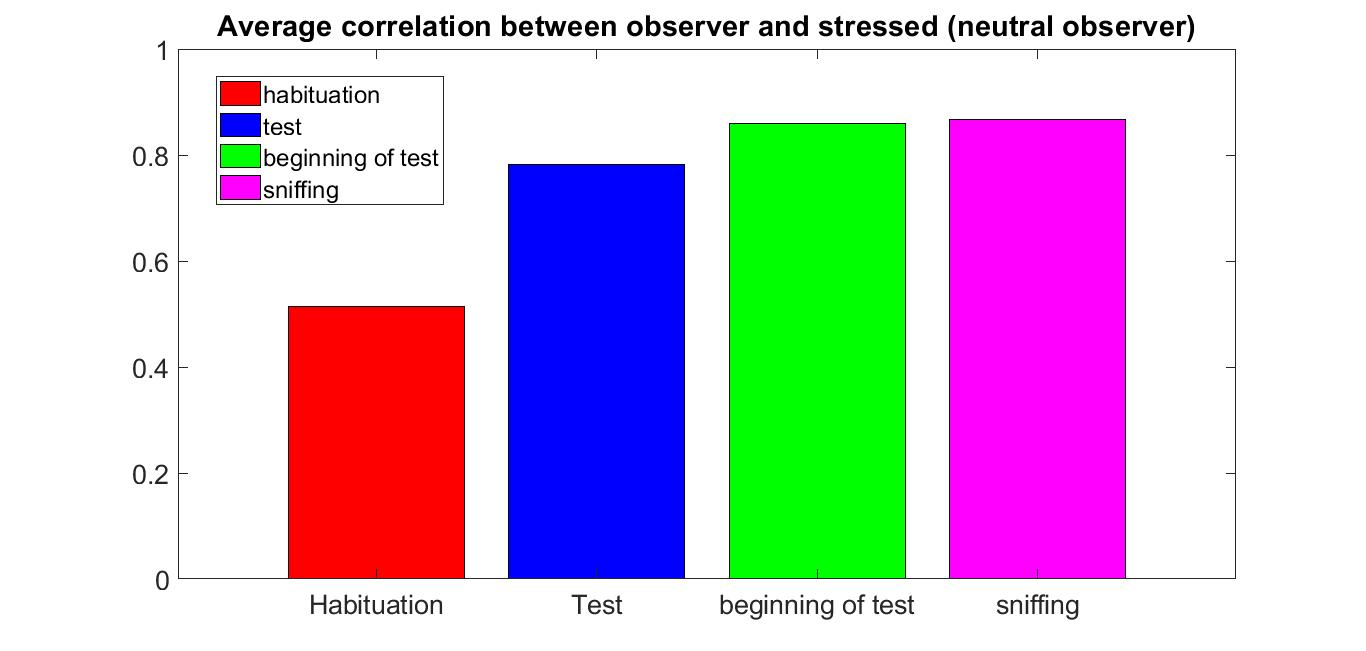
\includegraphics[scale=.32]{avg_corr_stress.jpg} 
	\end{center}  
	
	
\end{figure}

\end{frame}

\begin{frame}
\frametitle{ Average correlation between observer and stressed with stressed observer}



\begin{figure}[H]
	\begin{center}
		\hspace*{-1.7cm}
		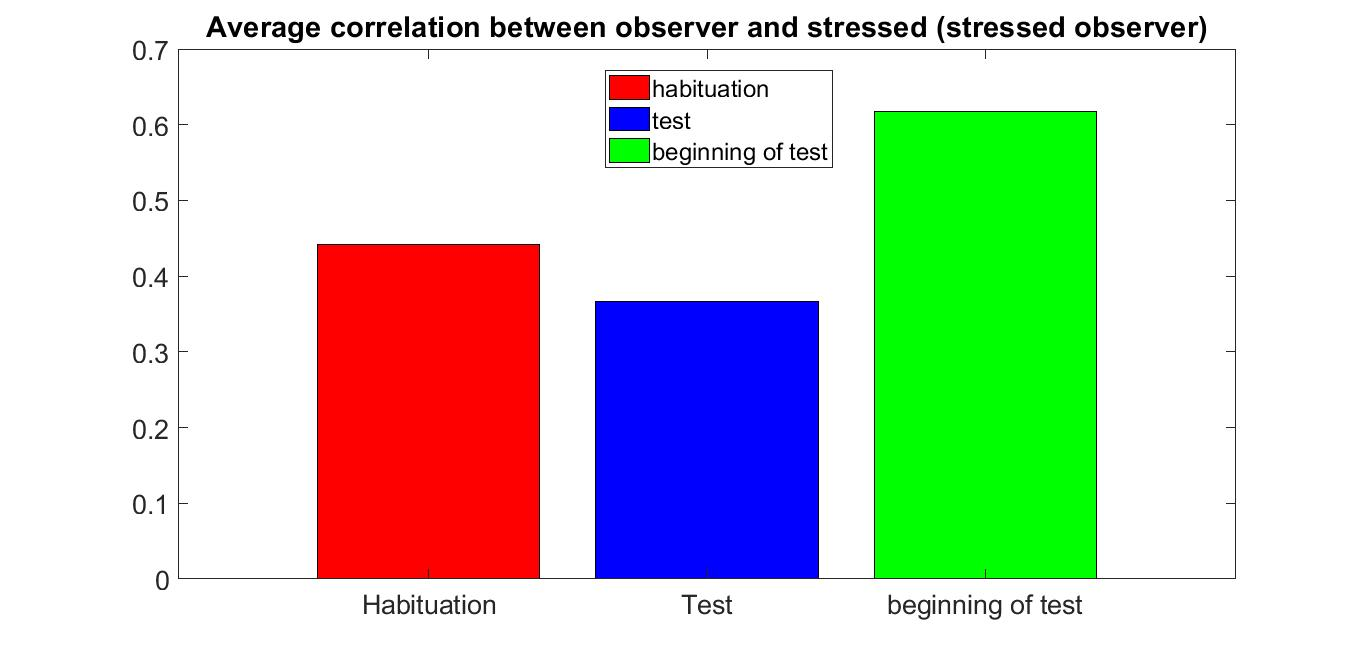
\includegraphics[scale=.32]{avg_corr_stress2.jpg} 
	\end{center}  
	
	
\end{figure}

\end{frame}

\begin{frame}
\frametitle{ Average correlation between observer and neutral with neutral observer}



\begin{figure}[H]
	\begin{center}
		\hspace*{-1.7cm}
		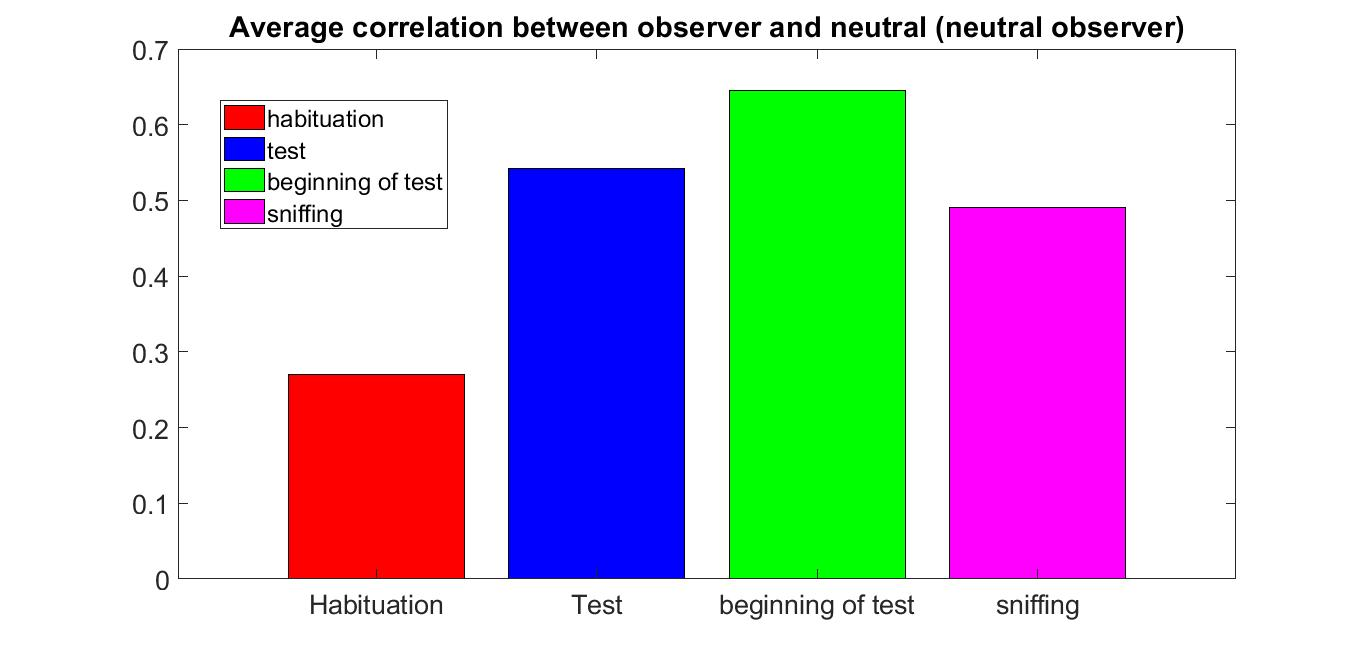
\includegraphics[scale=.32]{avg_corr_neut.jpg} 
	\end{center}  
	
	
\end{figure}

\end{frame}

\begin{frame}
\frametitle{ Average correlation between observer and neutral with stressed observer}



\begin{figure}[H]
	\begin{center}
		\hspace*{-1.7cm}
		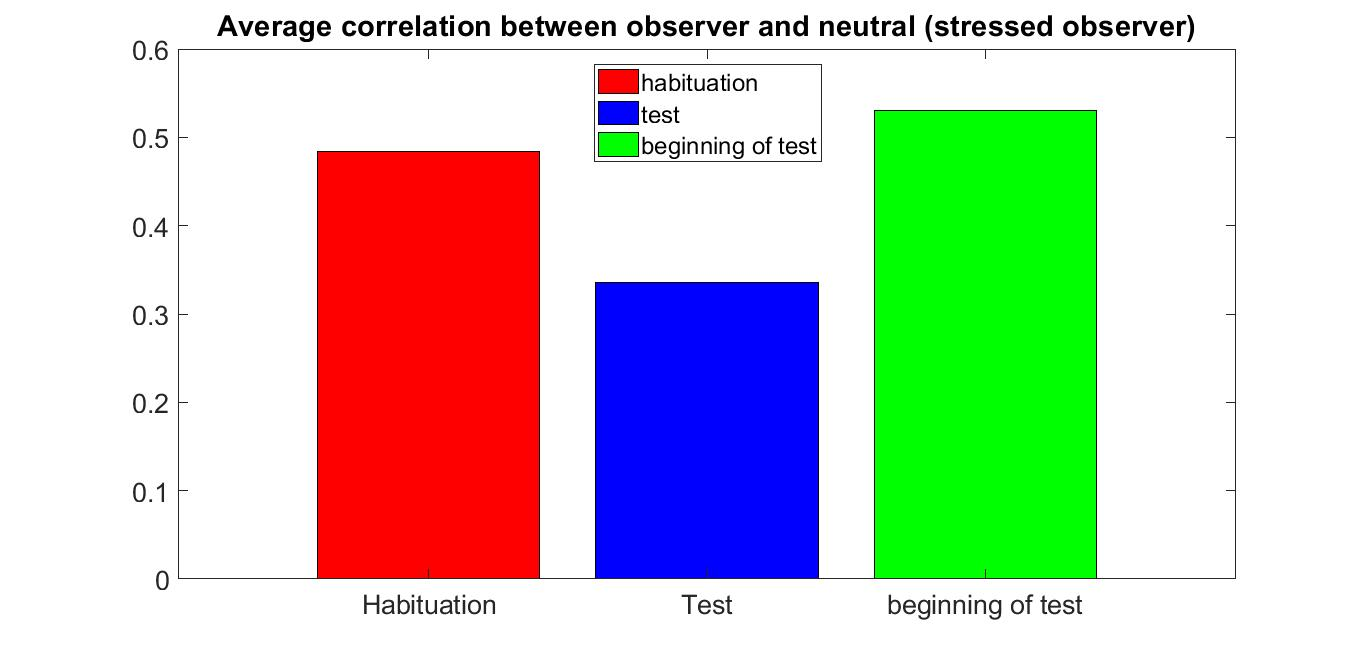
\includegraphics[scale=.32]{avg_corr_neut2.jpg} 
	\end{center}  
	
	
\end{figure}

\end{frame}


\begin{frame}
\frametitle{ Average correlation between pairs for observer and neutral}



\begin{figure}[H]
	\begin{center}
		\hspace*{-1.7cm}
		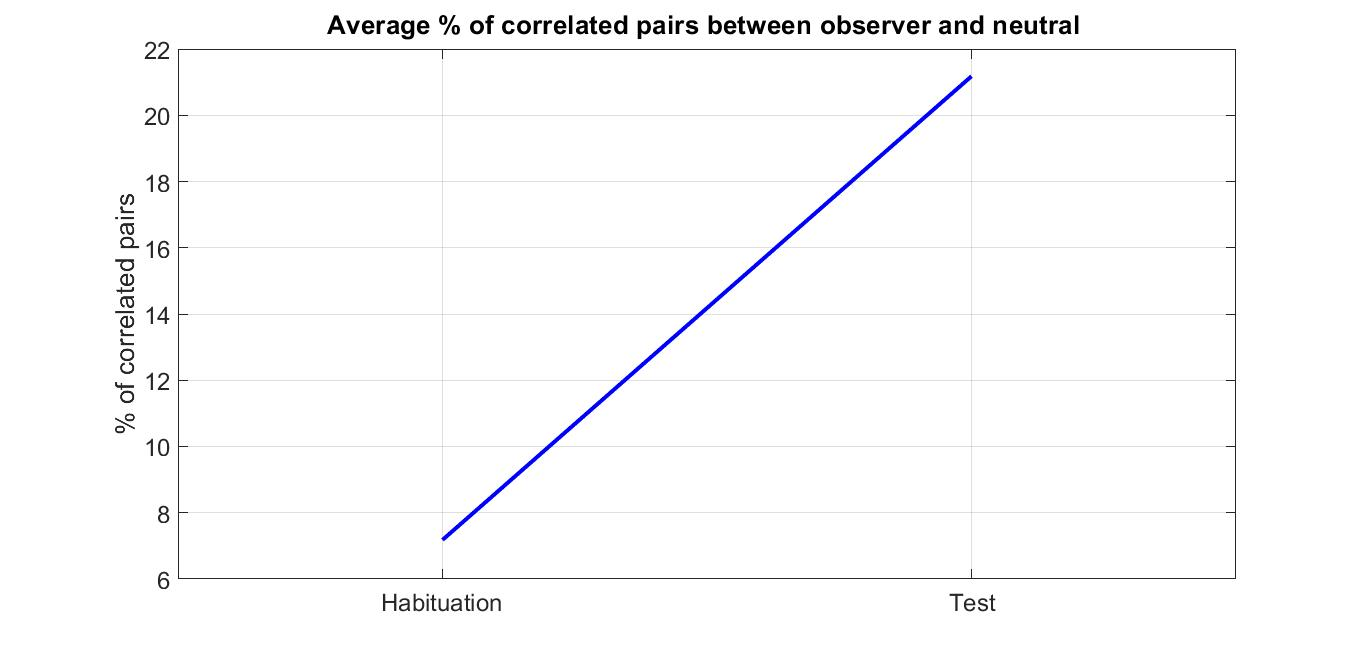
\includegraphics[scale=.32]{perc_neut.jpg} 
	\end{center}  
	
	
\end{figure}

\end{frame}

\begin{frame}
\frametitle{ Average correlation between pairs for observer and stressed}



\begin{figure}[H]
	\begin{center}
		\hspace*{-1.7cm}
		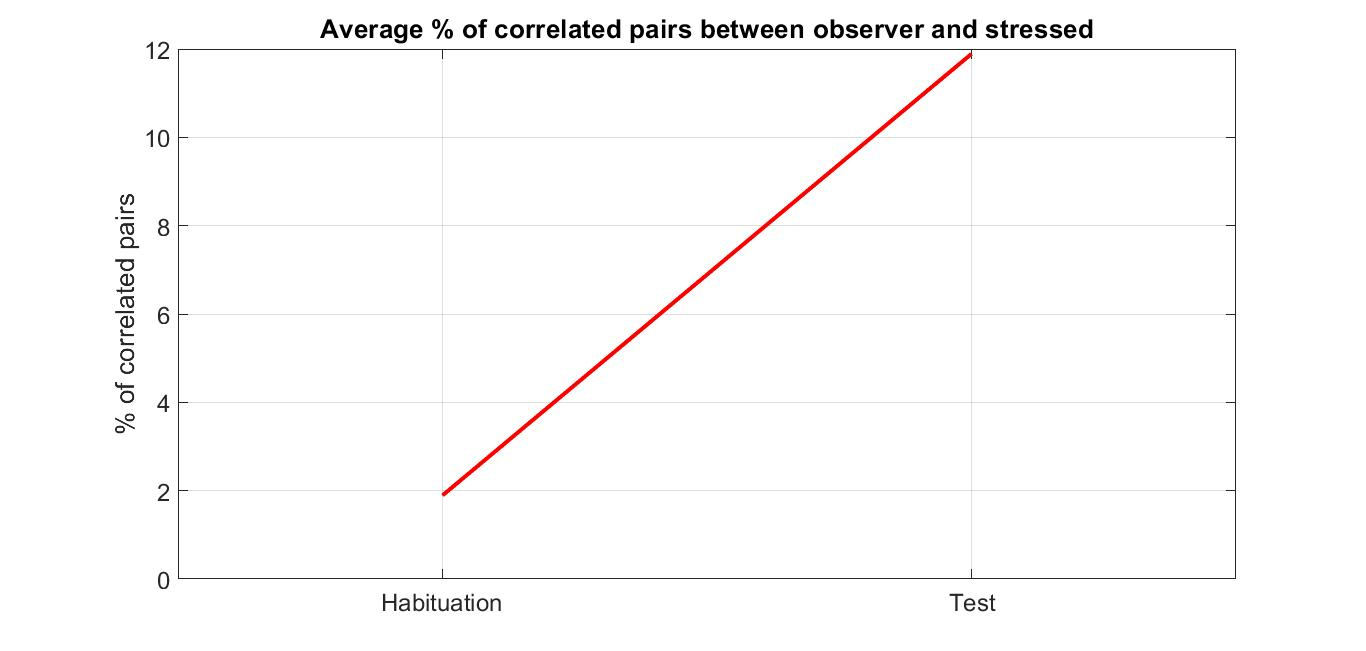
\includegraphics[scale=.32]{perc_stress.jpg} 
	\end{center}  
	
	
\end{figure}

\end{frame}


\begin{frame}
\frametitle{ Overall conclusions}



\begin{itemize}
	
	\item The average considerations on all data show an higher cross correlation recorded during the test phase than during the habituation, for both pairs observer/stressed and observer/neutral, with higher value in the first
	
	\item Such correlation is even higher if we restrict the analysis at the first part of the interactions
	
	\item Regarding the reciprocal  sniffing activity between mice, for the pair observer/stressed we have the highest correlation recorded
	
	\item $L^2$ and infinity errors between the recorded activities are in average smaller  during the test for the pair observer/stressed
	
	\item The percentage of correlated neurons for both pairs of mice is higher in the test

	
\end{itemize}

\end{frame}


\end{document}

\begin{frame}
\frametitle{}
\end{frame}